\documentclass{article}
\usepackage[utf8]{inputenc}

% Standard math packages
\usepackage{amsmath}
\usepackage{amsthm}
\usepackage{amssymb}
\usepackage{amsfonts}

% Other packages
\usepackage{scalerel}
\usepackage{stackengine}

% Packages for images
\usepackage{tikz}

% Package for the layout
\usepackage{geometry}

% Title Page
\title{Calculus}
\author{Jonathan Parker}
\date{Last Updated on \today}

% Counters
\renewcommand*\contentsname{Table of Contents}

\newtheorem{theorem}{Theorem}[section]

\newtheorem{definition}{Definition}[section]

\newtheorem{note}{Note}[section]

\newcounter{example}[section]
\newenvironment{example}[1][]{\refstepcounter{example}\par\medskip
   \noindent \textbf{Example~\theexample. #1} \rmfamily}{\medskip}

\newcounter{exercise}[section]
\newenvironment{exercise}[1][]{\refstepcounter{exercise}\par\medskip
   \noindent \textbf{Exercise~\theexercise. #1} \rmfamily}{\medskip}
   
\newcounter{recall}[section]
\newenvironment{recall}[1][]{\refstepcounter{recall}\par\medskip
   \noindent \textbf{Recall~\therecall. #1} \rmfamily}{\medskip}
   
% Declarations
\DeclareMathOperator*{\arccot}{arccot}
\DeclareMathOperator*{\arcsec}{arcsec}
\DeclareMathOperator*{\arccsc}{arccsc}
\DeclareMathOperator{\sgn}{sgn}

% Commands
\newcommand\showdiv[1]{\overline{\smash{\hstretch{.5}{)}\mkern-3.2mu\hstretch{.5}{)}}#1}}
\let\ph\phantom
   
% Removing indentations
\setlength{\parindent}{0pt}


\begin{document}

\maketitle
\tableofcontents

\newpage
\documentclass{article}
\usepackage[utf8]{inputenc}
\usepackage{amsmath}
\usepackage{amsthm}
\usepackage{amssymb}
\usepackage{geometry}
\usepackage{amsfonts} 

\title{Sequences of Numbers}
\author{Jonathan Parker}
\date{Last Updated on \today}

\renewcommand*\contentsname{Table of Contents}

\newtheorem{theorem}{Theorem}[section]

\newtheorem{definition}{Definition}[section]

\newtheorem{note}{Note}[section]

\newcounter{example}[section]
\newenvironment{example}[1][]{\refstepcounter{example}\par\medskip
   \noindent \textbf{Example~\theexample. #1} \rmfamily}{\medskip}

\newcounter{exercise}[section]
\newenvironment{exercise}[1][]{\refstepcounter{exercise}\par\medskip
   \noindent \textbf{Exercise~\theexercise. #1} \rmfamily}{\medskip}
   
\newcounter{recall}[section]
\newenvironment{recall}[1][]{\refstepcounter{recall}\par\medskip
   \noindent \textbf{Recall~\therecall. #1} \rmfamily}{\medskip}
   
\setlength{\parindent}{0pt}

\begin{document}


\maketitle
\tableofcontents

\newpage
\section{Introduction to Sequences of Numbers}\label{introduction_to_sequences_of_numbers}

\begin{definition}
A sequence of real numbers is a mapping
\begin{align*}
    f: \mathbb{N} \longrightarrow \mathbb{R}: f(n) \mapsto a_{n}
\end{align*}
We typically write the sequence in the following concise way:
\begin{align*}
    \{f(n)\}_{n=1}^{\infty} \hspace{20pt} \text{or} \hspace{20pt} \{a_{n}\}_{n=1}^{\infty}
\end{align*}
where $a_{n}$ is the real number function value at index $n$.
\end{definition}

\begin{example}
\begin{align*}
    &\Big\{\dfrac{1}{n}\Big\}_{n=1}^{\infty}\\[2ex]
    = \hspace{4pt} &\Big\{\dfrac{1}{1}, \hspace{4pt} \dfrac{1}{2}, \hspace{4pt} \dfrac{1}{3}, \hspace{4pt} \cdots \Big\}
\end{align*}
Here, $f(n) = \dfrac{1}{n}$ is the function definition from the natural numbers $\mathbb{N}$ to the real numbers $\mathbb{R}$.
\end{example}

\begin{exercise}
Write the $5^{\text{th}}$ term for the following sequence of real numbers:
\begin{align*}
    \Big\{\dfrac{n}{n+1}\Big\}_{n=1}^{\infty}
\end{align*}
\end{exercise}

\begin{exercise}
Write the first five terms for the following sequence of real numbers:
\begin{align*}
    \Big\{\dfrac{(-1)^{n}(n+1)}{3^{n}}\Big\}_{n=1}^{\infty}
\end{align*}
\end{exercise}

Sometimes, the domain is extended or attenuated a bit to accommodate the function definition.

\begin{exercise}
Write the first five terms for the following sequence of real numbers:
\begin{align*}
    \{\sqrt{n-10}\}_{n=10}^{\infty}
\end{align*}
\end{exercise}

\begin{exercise}
Write the first five terms for the following sequence of real numbers:
\begin{align*}
    \Big\{\cos{\Big(\dfrac{n\pi}{4}\Big)}\Big\}_{n=0}^{\infty}
\end{align*}
\end{exercise}

A tricky part of this concept is using a sequence's function values to determine the general formula.

\begin{example}
Let's take the following sequence of terms:
\begin{align*}
    \Big\{\dfrac{3}{5}, \hspace{4pt} -\dfrac{4}{25}, \hspace{4pt} \dfrac{5}{125}, \hspace{4pt} -\dfrac{6}{625}, \hspace{4pt} \dfrac{7}{3125}, \hspace{4pt} \cdots \Big\}
\end{align*}
Our job is to discover a pattern. Well, it seems every other term is negative. We know this can be established with the factor $(-1)^{n}$, but given that there are other factors we've yet to analyze thoroughly, it's not certain that this is a factor in our general expression for the sequence. It also seems the numerator begins at $3$ and increments by one unit as the sequence progresses. Given that the sequence begins at $n=3$, will our first term in the sequence be positive? We see $(-1)^{3}$ is negative. So, we fix this by adding or subtracting a $1$ from the power $n$. While it is not always the case that either adding or subtracting a $1$ will work, in this example, either approach will. So, we add a $1$, giving us $(-1)^{n+1}$ as a factor in our general sequence. Finally, the denominator seems to be some power of $5$ in each term of the sequence, and it seems those powers begin at $1$, which is equal to $3-2$. Checking the power in our second term, we have a power of $2$, which is equal to $4-2$. It seems our powers progress through the expression $n-2$, where $n$ is the index of the sequence. Thus, we have the following general expression for our sequence:
\begin{align*}
    \Big\{\dfrac{(-1)^{n+1}n}{5^{n-2}}\Big\}_{n=3}^{\infty}
\end{align*}
\end{example}

\begin{exercise}
Find the general expression of the sequence following the pattern:
\begin{align*}
    \Big\{1, \hspace{4pt} -\dfrac{2}{3}, \hspace{4pt} \dfrac{4}{9}, \hspace{4pt} -\dfrac{8}{27}, \hspace{4pt} \cdots \Big\}
\end{align*}
\end{exercise}

\newpage
\section{Limits of Sequences of Numbers}\label{limits_of_sequences_of_numbers}

\begin{definition}
A sequence $\{f(n)\}_{n=1}^{\infty}$ has a limit $L$, which we denote as 
\begin{align*}
    \lim_{n \longrightarrow \infty} f(n) = L\\[2ex]
    \text{if for all} \hspace{4pt} \epsilon > 0 \hspace{4pt} \text{there exists a natural number} \hspace{4pt} &N \hspace{4pt} \text{such that for all} \hspace{4pt} n \geq N \hspace{4pt} \text{we have}\\[2ex]
    \lvert f(n) - L \rvert < \epsilon
\end{align*}
Any sequence with a limit can be referred to as convergent.
\label{definition_limit_sequence_numbers}
\end{definition}

\begin{example}
$\lim_{n \longrightarrow \infty} \dfrac{1}{n} = 0$
\begin{proof}
Take $\epsilon = \dfrac{1}{k}$, where $k \in \mathbb{N}$ is arbitrary. Then by Definition \ref{definition_limit_sequence_numbers} we have
\begin{align*}
    &\Big\lvert \dfrac{1}{k+n} - 0 \Big\rvert\\[2ex]
    &= \Big\lvert \dfrac{1}{k+n} \Big\rvert\\[2ex]
    &< \dfrac{1}{k} = \epsilon, \hspace{4pt} \text{for all} \hspace{4pt} n \in \mathbb{N}
\end{align*}
\end{proof}
\label{limit_one_over_n}
\end{example}

\begin{theorem}
If $\{f(n)\}_{n=1}^{\infty}$ and $\{g(n)\}_{n=1}^{\infty}$ are convergent sequences, and if $c \in \mathbb{R}$, then
\begin{align*}
    &\lim_{n \longrightarrow \infty} (f(n) + g(n)) = \lim_{n \longrightarrow \infty} f(n) + \lim_{n \longrightarrow \infty} g(n) \\[2ex]
    &\lim_{n \longrightarrow \infty}(f(n) - g(n)) = \lim_{n \longrightarrow \infty} f(n) - \lim_{n \longrightarrow \infty} g(n)\\[2ex]
    &\lim_{n \longrightarrow \infty} cf(n) = c\lim_{n \longrightarrow \infty} f(n)\\[2ex]
    &\lim_{n \longrightarrow \infty} (f(n) \cdot g(n)) = \lim_{n \longrightarrow \infty} f(n) \cdot \lim_{n \longrightarrow \infty} g(n)\\[2ex]
    &\lim_{n \longrightarrow \infty}\dfrac{f(n)}{g(n)} = \dfrac{\lim_{n \longrightarrow \infty} f(n)}{\lim_{n \longrightarrow \infty} g(n)}, \hspace{4pt} \text{when} \hspace{4pt} \lim_{n \longrightarrow \infty} g(n) \neq 0\\[2ex]
    &\lim_{n \longrightarrow \infty} (f(n))^{p} = (\lim_{n \longrightarrow \infty} f(n))^{p}, \hspace{4pt} \text{where} \hspace{4pt} p > 0 \hspace{4pt} \text{and} \hspace{4pt} f(n) > 0\\[2ex]
    &\lim_{n \longrightarrow \infty} c = c
\end{align*}
\label{properties_limit_sequence_numbers}
\end{theorem}

Now that we have these result, we can use them to find limits of other sequences.

\begin{example}
$\lim_{n \longrightarrow \infty} \dfrac{n}{n+1} = 1$
\begin{proof}
We have a trick we can employ to find the above limit. By Example \ref{limit_one_over_n} and Theorem \ref{properties_limit_sequence_numbers},
\begin{align*}
    \dfrac{n}{n+1} &= 1 \cdot \dfrac{n}{n+1}
    = \dfrac{1/n}{1/n} \cdot \dfrac{n}{n+1}
    = \dfrac{(1/n) \cdot n}{(1/n) \cdot (n+1)}
    = \dfrac{1}{1 + (1/n)}\\[2ex]
    \Longrightarrow &\lim_{n \longrightarrow \infty} \dfrac{n}{n+1}
    = \lim_{n \longrightarrow \infty} \dfrac{1}{1+(1/n)}
    = \dfrac{\lim_{n \longrightarrow \infty}1}{\lim_{n \longrightarrow \infty}1 + \lim_{n \longrightarrow \infty}(1/n)}
    = \dfrac{1}{1 + 0} = 1
\end{align*}
\end{proof}
\end{example}

\begin{exercise}
Find the limit of 
\begin{align*}
    \Big\{\dfrac{n^{3}}{n^{3}+1}\Big\}_{n=1}^{\infty}
\end{align*}
\end{exercise}

\begin{exercise}
Find the limit of 
\begin{align*}
    \Big\{\dfrac{3+5n^{2}}{n+n^{2}}\Big\}_{n=1}^{\infty}
\end{align*}
\end{exercise}

\begin{exercise}
Find the limit of 
\begin{align*}
    \{e^{1/n}\}_{n=1}^{\infty}
\end{align*}
\end{exercise}

\begin{exercise}
Find the limit of
\begin{align*}
    \Big\{\tan\Big(\dfrac{2n\pi}{1+8n}\Big)\Big\}_{n=1}^{\infty}
\end{align*}
\end{exercise}

\begin{exercise}
Find the limit of
\begin{align*}
    \Big\{\sqrt{\dfrac{n+1}{9n+1}}\Big\}_{n=1}^{\infty}
\end{align*}
\end{exercise}

\begin{definition}
Take a sequence $\{f(n)\}_{n=1}^{\infty}$ 
\begin{align*}
    \text{If} \hspace{4pt} \lim_{n \longrightarrow \infty} f(n) &= \infty, \hspace{4pt} \text{then}\\[2ex]
    \text{for all} \hspace{4pt} N \in \mathbb{N}, \hspace{4pt} \text{there exists an} \hspace{4pt} M \in \mathbb{N} \hspace{4pt} &\text{such that for all} \hspace{4pt} n > M \hspace{4pt} \text{we have} \hspace{4pt} f(n) > N.
\end{align*}
\begin{align*}
    \text{If} \hspace{4pt} \lim_{n \longrightarrow \infty} f(n) &= -\infty, \hspace{4pt} \text{then}\\[2ex]
    \text{for all} \hspace{4pt} N \in \mathbb{N}, \hspace{4pt} \text{there exists an} \hspace{4pt} M \in \mathbb{N} \hspace{4pt} &\text{such that for all} \hspace{4pt} n > M \hspace{4pt} \text{we have} \hspace{4pt} f(n) < -N.
\end{align*}
Any sequence with an infinite limit is said to be divergent.
\label{definition_infinite_limit_sequence}
\end{definition}

\begin{example}
Take $\{n\}_{n=1}^{\infty}$. Clearly, as $n \longrightarrow \infty$, the sequence of function values push to infinity.
\end{example}

\begin{exercise}
Show the sequence $\Big\{\dfrac{n^{3}}{n+1}\Big\}_{n=1}^{\infty}$ has an infinite limit. 
\end{exercise}

\begin{exercise}
Show the sequence $\Big\{\dfrac{n!}{2^{n}}\Big\}_{n=1}^{\infty}$ has an infinite limit. 
\end{exercise}

\begin{theorem}
A sequence of numbers can have at most one limit.
\label{limit_uniqueness}
\end{theorem}

\begin{note}
Any sequence that does not converge to a single, finite value is considered divergent.
\end{note}

\begin{exercise}
Find the general expression of the divergent sequence following the pattern:
\begin{align*}
    \{5, \hspace{4pt} 1, \hspace{4pt} 5, \hspace{4pt} 1, \hspace{4pt} 5, \hspace{4pt} 1, \hspace{4pt} \cdots\}
\end{align*}
\end{exercise}

\begin{exercise}
Find the general expression of the divergent sequence following the pattern:
\begin{align*}
    \{2, \hspace{4pt} 7, \hspace{4pt} 12, \hspace{4pt} 17, \hspace{4pt} \cdots\}
\end{align*}
\end{exercise}

\begin{exercise}
Determine whether the sequence defined by the following is convergent or divergent:
\begin{align*}
    f(1) = 1 \hspace{20pt} f(n) = 4 - f(n-1), \hspace{20pt} n \geq 1
\end{align*}
\end{exercise}

\begin{exercise}
Determine whether the sequence defined by the following is convergent or divergent:
\begin{align*}
    f(1) = 2 \hspace{20pt} f(n) = 4 - f(n-1), \hspace{20pt} n \geq 1
\end{align*}
\end{exercise}

\begin{recall}
For all $a, b \in \mathbb{R}$, we have
\begin{align*}
    \Big\lvert \lvert a \rvert - \lvert b \rvert \Big\rvert &\leq \lvert a - b \rvert \\[2ex]
    \lvert a + b \rvert &\leq \lvert a \rvert + \lvert b \rvert
\end{align*}
\end{recall}



\end{document}


\newpage
\section{Limits of Functions}

\begin{definition}
We say $f$ as a function of $x$ has a limit $L$ at $c \in \mathbb{R}$, denoted by
\begin{align*}
    &\lim_{x \longrightarrow c} f(x) = L \hspace{4pt} \text{if} \hspace{20pt} &&\text{for all} \hspace{4pt} \epsilon > 0, \hspace{4pt} \text{there exists a} \hspace{4pt} \delta > 0 \hspace{4pt} \text{such that}\\[2ex]
    &\text{for all} \hspace{4pt} x \in \text{Dom($f$)} \hspace{4pt} \text{satisfying} \hspace{4pt} \lvert x - c \rvert < \delta &&\text{we have} \hspace{4pt} \lvert f(x) - L \rvert < \epsilon
\end{align*}
\end{definition}





\newpage
\section{Continuity of Functions}

\begin{definition}
We say a function $f$ is continuous at a point $c \in \text{Dom($f$)}$ if
\begin{align*}
    &\text{For any} \hspace{4pt} \epsilon > 0, \hspace{4pt} \text{there exists a} \hspace{4pt} \delta > 0 \hspace{4pt} \text{such that}\\[2ex]
    &\text{for any} \hspace{4pt} x \hspace{4pt} \text{satisfying} \hspace{4pt} \lvert x - c \rvert < \delta \hspace{20pt} \text{we have} \hspace{20pt} \lvert f(x) - f(c) \rvert < \epsilon
\end{align*}
This is equivalent to saying $\lim_{x \longrightarrow c} f(x) = f(c)$ when $f$ is continuous at $c$. For continuity to hold, we need three things to be true:
\begin{itemize}
    \item $f$ is defined at $c$. Meaning, $f(c)$ must exist.\\
    \item $\lim_{x \longrightarrow c} f(x)$ must exist.\\
    \item $lim_{x \longrightarrow c} f(x) = f(c)$
\end{itemize}
In fact, the definition of continuity is almost exactly the same as the definition of a limit, Definition \ref{definition_limit_of_functions} in section \ref{limits_of_functions_section}.
\label{definition_function_continuity}
\end{definition}

\begin{exercise}
What is the difference between the definition of the limit of a function, Definition \ref{definition_limit_of_functions} in section \ref{limits_of_functions_section}, and the definition of continuity of a function, Definition \ref{definition_function_continuity}?
\end{exercise}

\begin{theorem}
If $f$ is continuous at $c$, then $f$ has a limit at $c$.
\end{theorem}

\begin{exercise}
TRUE or FALSE: If $f$ is not continuous at $c$ (we say $f$ is discontinuous when $f$ is not continuous) then $f$ does not have a limit at $c$.
\end{exercise}

\begin{definition}
We say a function $f$ is continuous on Dom($f$) if for every $c \in \text{Dom($f$)}$ we have 
\begin{align*}
    &\text{For any} \hspace{4pt} \epsilon > 0, \hspace{4pt} \text{there exists a} \hspace{4pt} \delta > 0 \hspace{4pt} \text{such that}\\[2ex]
    &\text{for any} \hspace{4pt} x \hspace{4pt} \text{satisfying} \hspace{4pt} \lvert x - c \rvert < \delta \hspace{20pt} \text{we have} \hspace{20pt} \lvert f(x) - f(c) \rvert < \epsilon
\end{align*}
\end{definition}

\begin{example}
Revisiting our example from earlier, Example \ref{limit_of_sin_0_1} in section \ref{limits_of_functions_section}, we discovered that $f(x) = \sin x$, where $x$ belongs to the interval $[0, 1]$, has a limit at $c=1/2$. Since $f$ is defined at $c=1/2$, we also have
\begin{align*}
    \lim_{x \longrightarrow 1/2} f(x) = f\Big(\dfrac{1}{2}\Big) = \sin \Big(\dfrac{1}{2}\Big)
\end{align*}
Since the sine function is defined at every point of the real line, 
\begin{align*}
    \lim_{x \longrightarrow c} \sin x = \sin c \hspace{20pt} \text{for all} x \in \mathbb{R}
\end{align*}

\resizebox{30em}{30em}{%
\begin{tikzpicture}[scale=\textwidth/4.2cm]
    % title and axes
    \node at (0.7, 1.1) {\tiny$f(x)=\sin x \hspace{4pt} x \in \Big[0, 1 \Big]$};
    \draw (0, 0) -- (1, 0)
        node[right] {\tiny$x$};
    \draw (0, 0) -- (0, 1)
        node[above] {\tiny$f(x)$};
    % ----------------------------------
    % range boundaries lower
    \draw[dotted] (0, {sin(0.45 r)}) -- (0.6, {sin(0.45 r)});
    \node[] at (-0.15, {sin(0.45 r)}) {\tiny$L-\epsilon$};
    \node [rotate=90] at (0, {sin(0.45 r)}) {\tiny(};
    % range boundaries upper
    \draw[dotted] (0, {sin(0.55 r)}) -- (0.6, {sin(0.55 r)});
    \node[] at (-0.15, {sin(0.55 r)}) {\tiny$L+\epsilon$};
    \node [rotate=-90] at (0, {sin(0.55 r)}) {\tiny(};
    % ----------------------------------
    % domain boundaries lower
    \draw[dotted] (0.47, 0) -- (0.47, {sin(0.6 r)});
    \node [rotate=45] at (0.35, -0.15) {\tiny$\dfrac{1}{2}-\delta$ $\longrightarrow$};
    \node [] at (0.47, 0) {\tiny(};
    % domain boundaries upper
    \draw[dotted] (0.53, 0) -- (0.53, {sin(0.6 r)});
    \node [rotate=-45] at (0.65, -0.15) {\tiny$\longleftarrow$ \tiny$\dfrac{1}{2}+\delta$};
    \node [] at (0.53, 0) {\tiny)};
    % ----------------------------------
    % graph
    \draw[blue] plot[smooth] file {limits_of_functions/python_generated_tables/sine_0_1_piece_0.table};
    \draw[blue] plot[smooth] file {limits_of_functions/python_generated_tables/sine_0_1_piece_1.table};
    \draw[blue, fill=red] (0.5,{sin(0.5 r)}) circle (.25mm);
\end{tikzpicture}
}
\end{example}

\begin{recall}
From section \ref{limits_of_functions_section}, we stated that 
\begin{align*}
    \lim_{x \longrightarrow c} x = c \hspace{4pt} \text{for all} x \in \mathbb{R} \hspace{20pt} \text{when} \hspace{20pt} f(x) = x 
\end{align*}
This means that $f(x) = x$ is continuous on the real line. This fact brings us to another useful result:
\end{recall}

\begin{theorem}
Every polynomial $p$, defined formally by
\begin{align*}
    &p(x) = a_{n}x^{n} + a_{n-1}x^{n-1} + \cdots + a_{2}x^{2} + a_{1}x + a_{0}\\[2ex]
    &\text{where} \hspace{4pt} \{a_{n}, a_{n-1}, \cdots , a_{3}, a_{2}, a_{1}, a_{0}\} \hspace{4pt} \text{are all real numbers and} \hspace{4pt} a_{n} \neq 0
\end{align*}
is continuous on the real line. This, in turn, provides us with another useful result:
\end{theorem}

\begin{theorem}
Every rational function $R(x)=\dfrac{p(x)}{q(x)}$, where $p$ and $q$ are polynomials, is continuous for all real numbers $c$ such that $q(c) \neq 0$.
\end{theorem}

\begin{exercise}
Where along the real line is the following continuous:
\begin{align*}
    f(x) = \dfrac{x^{2}-x-2}{x-2}
\end{align*}
\end{exercise}

\begin{exercise}
Where along the real line is the following continuous:
\begin{align*}
    f(x) =
    \begin{cases}
    \dfrac{1}{x^{2}}, &x \neq 0\\
    1, &x = 0
    \end{cases}
\end{align*}
\end{exercise}

\begin{exercise}
Where along the real line is the following discontinuous:
\begin{align*}
    f(x) = 
    \begin{cases}
    \dfrac{x^{2}-x-2}{x-2}, &x \neq 2 \\
    1, & x=2
    \end{cases}
\end{align*}
\end{exercise}

\begin{definition}
We say a function $f$ is right-continuous if
\begin{align*}
    \lim_{x \longrightarrow c^{+}} f(x) = f(c)
\end{align*}
We say a function is left-continuous if
\begin{align*}
    \lim_{x \longrightarrow c^{-}} f(x) = f(c)
\end{align*}
\end{definition}

\begin{theorem}
A function $f$ is continuous if and only if
\begin{align*}
    \lim_{x \longrightarrow c^{-}} f(x) = f(c) = \lim_{x \longrightarrow c^{+}} f(x) 
\end{align*}
\end{theorem}

\begin{example}
Below is a visual of the floor function on the attenuated domain $[0, 2)$, with the open, white-colored circles depicting where a function is discontinuous from the left, and the closed, red-colored circles depicting where a function is continuous from the right. We see that $f$ is discontinuous at $1$:
\begin{align*}
    &\lim_{x \longrightarrow 1^{-}} \lfloor x \rfloor = 0 \hspace{20pt} \lim_{x \longrightarrow 1^{+}} \lfloor x \rfloor = 1\\[2ex]
    &\text{Since} \hspace{4pt} \lim_{x \longrightarrow 1^{-}} f(x) \neq f(1) \hspace{4pt} f \hspace{4pt} \text{is not continuous at} \hspace{4pt} 1
\end{align*}

\resizebox{30em}{30em}{%
\begin{tikzpicture}[scale=\textwidth/4.2cm]
    % title and axes
    \node at (1.3, 1.5) {$f(x)=\lfloor x \rfloor \hspace{4pt} x \in [0, 2)$};
    \draw (0, 0) -- (2, 0)
        node[right] {$x$};
    \draw (0, 0) -- (0, 1.3)
        node[above] {$f(x)$};
    % graph
    \draw[blue, very thick] plot[smooth] file {limits_of_functions/python_generated_tables/floor_0_2_piece_0.table};
    \draw[blue, very thick] plot[smooth] file {limits_of_functions/python_generated_tables/floor_0_2_piece_1.table};
    \draw[blue, fill=white] (1,0) circle (.25mm);
    \draw[blue, fill=white] (2,1) circle (.25mm);
    \draw[blue, fill=red] (0,0) circle (.25mm);
    \draw[blue, fill=red] (1,1) circle (.25mm);
    \node at (0, -0.1) {0};
    \node at (1, -0.1) {1};
    \node at (2, -0.1) {2};
\end{tikzpicture}
}
\end{example}

\begin{exercise}
For the floor function $f(x) = \lfloor x \rfloor$, for an arbitrary integer $n$, find
\begin{align*}
    &\lim_{x \longrightarrow n^{-}} f(x)\\
    &\lim_{x \longrightarrow n^{+}} f(x)
\end{align*}
\end{exercise}

\begin{example}
Here we have the ceiling function on the attenuated domain (-1, 1]:
\begin{align*}
    f(x) = \lceil x \rceil \hspace{20pt} x \in [-1, 1)
\end{align*}
We see that it is discontinuous at $0$:
\begin{align*}
    &\lim_{x \longrightarrow 0^{-}} \lceil x \rceil = 0 \hspace{20pt} \lim_{x \longrightarrow 0^{+}} \lceil x \rceil 1\\[2ex]
    &\text{Since} \hspace{4pt} \lim_{x \longrightarrow 0^{+}}f(x) \neq f(0) \hspace{4pt} f \hspace{4pt} \text{is discontinuous at} \hspace{4pt} 0
\end{align*}

\resizebox{30em}{30em}{%
\begin{tikzpicture}[scale=\textwidth/4.2cm]
    % title and axes
    \node at (0.6, 1.2) {$f(x)=\lceil x \rceil \hspace{4pt} x \in (-1, 1]$};
    \draw (-1, 0) -- (1, 0)
        node[right] {$x$};
    \draw (0, 0) -- (0, 1.3)
        node[above] {$f(x)$};
    % graph
    \draw[blue, very thick] plot[smooth] file {continuity_of_functions/python_generated_tables/ceiling_neg1_1_piece_0.table};
    \draw[blue, very thick] plot[smooth] file {continuity_of_functions/python_generated_tables/ceiling_neg1_1_piece_1.table};
    \draw[blue, fill=red] (0,0) circle (.25mm);
    \draw[blue, fill=red] (1,1) circle (.25mm);
    \draw[blue, fill=white] (-1,0) circle (.25mm);
    \draw[blue, fill=white] (0,1) circle (.25mm);
    \node at (-1, -0.1) {-1};
    \node at (0, -0.1) {0};
    \node at (1, -0.1) {1};
\end{tikzpicture}
}
\end{example}

\begin{exercise}
For the ceiling function $f(x) = \lceil x \rceil$, for an arbitrary integer $n$, find
\begin{align*}
    &\lim_{x \longrightarrow n^{-}} f(x)\\
    &\lim_{x \longrightarrow n^{+}} f(x)
\end{align*}
\end{exercise}

\newpage
\section{The Derivative}

\begin{definition}
We say a function $f$ has derivative $L$ at $c \in$ Dom($f$) if 
\begin{align*}
    &\text{For all} \hspace{4pt} \epsilon > 0 \hspace{4pt} \text{there exists a} \hspace{4pt} \delta > 0 \hspace{4pt} \text{such that}\\[2ex]
    &\text{all} \hspace{4pt} x \in \text{Dom($f$)} \hspace{4pt} \text{satisfying} \hspace{4pt} \lvert x-c \rvert < \delta \hspace{20pt} \Longrightarrow \hspace{20pt} \Big\lvert \dfrac{f(x)-f(c)}{x-c}-L \Big\rvert < \epsilon
\end{align*}
We denote $L$ as
\begin{align*}
f^{'}(c) = \lim_{x \longrightarrow c} \dfrac{f(x)-f(c)}{x-c}
\end{align*}
which can be written equivalently as
\begin{align*}
    f^{'}(c) = \lim_{h \longrightarrow 0} \dfrac{f(c+h)-f(c)}{h}
\end{align*}
\end{definition}

\begin{example}
The derivative of a function $f$ at a point $c \in$ Dom($f$) can be thought of as the slope of the linear function $L(x)$ tangent to function $f$ at point $c$. The slope of a $1$-D line in $2$-D space is what we will deal with most in this course, but the slope of a $2$-D plane in $3$-D space or the slope of a $(n-1)$-D plane in $n$-D space can also be a derivative of some function in these respective spaces. Below, we show a subset of the secant lines (in black) passing through the point $(\pi/4, \sqrt{2}/2)$, all of which can be formed as we push towards the derivative (tangent line in red) passing through the point $(\pi/4, \sqrt{2}/2)$.
\begin{align*}
    &\text{When} \hspace{4pt} f(x) = \sin x\\[2ex]
    &\text{and when} \hspace{4pt} f^{'}\Big(\dfrac{\pi}{4}\Big) = \lim_{h \longrightarrow 0} \dfrac{\sin\Big(\dfrac{\pi}{4} + h\Big) - \sin\Big(\dfrac{\pi}{4}\Big)}{h}\\[2ex]
    &\text{then we have the tangent line} \hspace{4pt} L(x) = (f^{'}(x))x + b \hspace{20pt}\\[2ex]
    &\text{where $b$ is the intercept of the linear function $L$}
\end{align*}

\resizebox{30em}{30em}{%
\begin{tikzpicture}[scale=\textwidth/4.2cm]
    % title and axes
    \node at (0.6, 1.2) {$f(x)=\sin x \hspace{4pt} x \in [0, \pi]$};
    \draw (0, 0) -- (pi, 0)
        node[right] {$x$};
    \draw (0, 0) -- (0, 2.4)
        node[above] {$f(x)$};
    % graph
    \draw[red, very thick] plot[smooth] file {derivatives_of_functions/python_generated_tables/sin_0_pi_tangent.table};
    \draw[black] plot[smooth] file {derivatives_of_functions/python_generated_tables/sin_0_pi_line_5.table};
    \draw[black] plot[smooth] file {derivatives_of_functions/python_generated_tables/sin_0_pi_line_6.table};
    \draw[blue, very thick] plot[smooth] file {derivatives_of_functions/python_generated_tables/sin_0_pi.table};
    \draw[black] plot[smooth] file {derivatives_of_functions/python_generated_tables/sin_0_pi_line_1.table};
    \draw[black] plot[smooth] file {derivatives_of_functions/python_generated_tables/sin_0_pi_line_2.table};
    \draw[black] plot[smooth] file {derivatives_of_functions/python_generated_tables/sin_0_pi_line_3.table};
    \draw[black] plot[smooth] file {derivatives_of_functions/python_generated_tables/sin_0_pi_line_4.table};
    \draw[blue, fill=red] (pi/4, {sqrt(2)/2}) circle (.25mm);
    \draw[black, fill=black] (2*pi/3, {sqrt(3)/2}) circle (.25mm);
    \draw[black, fill=black] (pi/2, 1) circle (.25mm);
    \node at (pi/4, -0.1) {$\pi/4$};
    \node at (2*pi/3, -0.1) {$2\pi/3$};
    \node at (pi/2, -0.1) {$\pi/2$};
    \draw[dotted] (pi/4, 0) -- (pi/4, {sqrt(2)/2});
    \draw[dotted] (pi/2, 0) -- (pi/2, 1);
    \draw[dotted] (2*pi/3, 0) -- (2*pi/3, {sqrt(3)/2});
\end{tikzpicture}
}
\end{example}

\newpage
\section{The Riemann Integral}

\begin{definition}
Let $I = [a, b]$, where $a$ and $b$ are real numbers, be a subset of $\mathbb{R}$ and let 
\begin{align*}
    P = \{x_{0}, x_{1}, x_{2}, ..., x_{n-1}, x_{n}\} \hspace{20pt} \text{such that} \hspace{20pt} a = x_{0} < x_{1} < x_{2} < \cdots < x_{n-1} < x_{n} = b
\end{align*}
be a finite subset of numbers contained in $I$. Take each member $x_{i}$ of $P$ and use it to create a sub-interval $I_{i}$ of $I$, such that the union of these sub-intervals is $I$, as follows
\begin{align*}
    I_{0} = [x_{0}, x_{1}) \hspace{20pt} I_{1} = [x_{1}, x_{2})& \hspace{20pt} \cdots \hspace{20pt} I_{n-2} = [x_{n-2}, x_{n-1}) \hspace{20pt} I_{n-1} = [x_{n-1}, x_{n}]\\[2ex]
    &I = I_{0} \cup I_{1} \cup I_{2} \cup \cdots \cup I_{n-2} \cup I_{n-1}
\end{align*}
From each $I_{i}$, choose a number $t_{i}$. We call the following set of ordered pairs a tagged partition
\begin{align*}
    \dot P = \{ \hspace{4pt} ( \hspace{4pt} [x_{i}, x_{i+1}), t_{i} \hspace{4pt} ) \hspace{4pt}\}_{i = 0}^{n-2} \hspace{10pt} \cup \hspace{10pt} \{ \hspace{4pt} ( \hspace{4pt} [x_{n-1}, x_{n}], t_{n-1} \hspace{4pt} ) \hspace{4pt} \}
\end{align*}
\end{definition}

\begin{definition}
The norm of a tagged partition is defined as
\begin{align*}
    \lvert \lvert \dot P \rvert \rvert = \max \{x_{1} - x_{0}, x_{2} - x_{1}, \cdots , x_{n-1} - x_{n-2}, x_{n} - x_{n-1}\}
\end{align*}
\end{definition}

\begin{definition}
A function $f$ on $I=[a, b]$ is said to be Riemann integrable on $[a, b]$ if there exists a real number $L$ such that for every $\epsilon > 0$ there exists a $\delta > 0$ satisfying the following
\begin{align*}
    &\text{whenever} \hspace{4pt} \dot P \hspace{4pt} \text{is a tagged partition of $[a, b]$}\\[2ex]
    &\text{if} \hspace{20pt} \lvert \lvert \dot P \rvert \rvert < \delta \hspace{20pt} \text{then} \hspace{20pt} \Big\lvert \sum_{i=0}^{n-1} f(t_{i})(x_{i+1} - x_{i}) - L \Big\rvert < \epsilon  
\end{align*}
For this course, we will use the following notation for $L$
\begin{align*}
    L = \int_{a}^{b} f(x) dx
\end{align*}
\end{definition}

\begin{example}
This is an example of a Riemann sum. There are infinitely many tagged partitions we could use for any example, all of which are merely an approximation of the integral of the function, except in the limit. We've chosen one that demonstrates the flexibility of these partitions. Notice that the widths of the rectangles are visibly different, and notice the visible difference in where $t_{i}$ is positioned for each interval. This particular partition for the function $f$ can be written as
\begin{align*}
    \dot P = \{ \hspace{4pt} ( \hspace{4pt} [x_{i}, x_{i+1}), t_{i} \hspace{4pt} ) \hspace{4pt} \}_{i = 0}^{6} \hspace{10pt} \cup \hspace{10pt} \{ \hspace{4pt} ( \hspace{4pt} [x_{7}, x_{8}], t_{7} \hspace{4pt} ) \hspace{4pt} \} \hspace{20pt} \text{where} \hspace{20pt} f(x) = \cos x \hspace{20pt} x \in [0, 1]  
\end{align*}
So, for our partition, we have the endpoints
\begin{align*}
    x_{0} = 0 \hspace{20pt} \text{and} \hspace{20pt} x_{8} = 1
\end{align*}
\resizebox{30em}{30em}{%
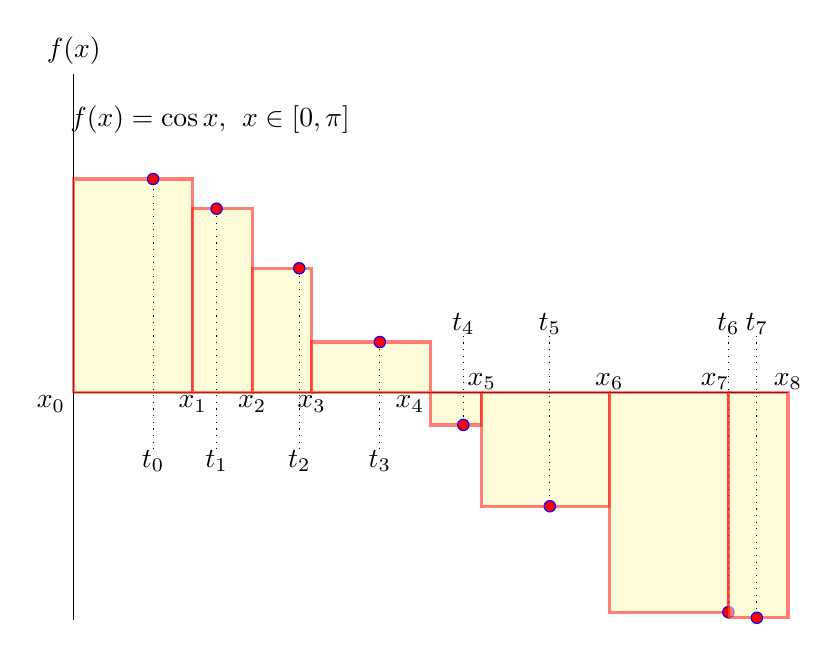
\begin{tikzpicture}[scale=\textwidth/4.2cm]
    % title and axes
    \node at (0.6, 1.2) {$f(x)=\cos x, \hspace{4pt} x \in [0, \pi]$};
    \draw (0, 0) -- (pi, 0);
    \draw (0, 0) -- (0, 1.4)
        node[above] {$f(x)$};
    \draw (0, 0) -- (0, -1);
    % graph
    \draw[black, very thick] plot[smooth] file {integrals_of_functions/python_generated_tables/cos_0_pi_riemann_sum.table};
    \draw[red, very thick, fill=yellow!30, opacity=0.5] (0, 0) 
        -- (pi/6, 0)
        -- (pi/6, {cos(pi/9 r)})
        -- (0, {cos(pi/9 r)})
        -- (0, 0);
    \node at (-0.1, -0.05) {$x_{0}$};
    \node at (pi/9, -0.3) {$t_{0}$};
    \node at (pi/6, -0.05) {$x_{1}$};
    \draw[black, dotted] (pi/9, -0.25) -- (pi/9, {cos(pi/9 r)});
    \draw[blue, fill=red] (pi/9, {cos(pi/9 r)}) circle (.25mm);
    \draw[red, very thick, fill=yellow!30, opacity=0.5] (pi/6, 0) 
        -- (pi/4, 0)
        -- (pi/4, {cos(pi/5 r)})
        -- (pi/6, {cos(pi/5 r)})
        -- (pi/6, 0);
    \node at (pi/5, -0.3) {$t_{1}$};
    \node at (pi/4, -0.05) {$x_{2}$};
    \draw[black, dotted] (pi/5, -0.25) -- (pi/5, {cos(pi/5 r)});
    \draw[blue, fill=red] (pi/5, {cos(pi/5 r)}) circle (.25mm);
    \draw[red, very thick, fill=yellow!30, opacity=0.5] (pi/4, 0) 
        -- (pi/3, 0)
        -- (pi/3, {cos(12*pi/38 r)})
        -- (pi/4, {cos(12*pi/38 r)})
        -- (pi/4, 0);
    \node at (12*pi/38, -0.3) {$t_{2}$};
    \node at (pi/3, -0.05) {$x_{3}$};
    \draw[black, dotted] (12*pi/38, -0.25) -- (12*pi/38, {cos(12*pi/38 r)});
    \draw[blue, fill=red] (12*pi/38, {cos(12*pi/38 r)}) circle (.25mm);
    \draw[red, very thick, fill=yellow!30, opacity=0.5] (pi/3, 0) 
        -- (pi/2, 0)
        -- (pi/2, {cos(12*pi/28 r)})
        -- (pi/3, {cos(12*pi/28 r)})
        -- (pi/3, 0);
    \node at (12*pi/28, -0.3) {$t_{3}$};
    \node at (8*pi/17, -0.05) {$x_{4}$};
    \draw[black, dotted] (12*pi/28, -0.25) -- (12*pi/28, {cos(12*pi/28 r)});
    \draw[blue, fill=red] (12*pi/28, {cos(12*pi/28 r)}) circle (.25mm);
    \draw[red, very thick, fill=yellow!30, opacity=0.5] (pi/2, 0) 
        -- (4*pi/7, 0)
        -- (4*pi/7, {cos(6*pi/11 r)})
        -- (pi/2, {cos(6*pi/11 r)})
        -- (pi/2, 0);
    \node at (6*pi/11, 0.3) {$t_{4}$};
    \node at (4*pi/7, 0.05) {$x_{5}$};
    \draw[black, dotted] (6*pi/11, 0.25) -- (6*pi/11, {cos(6*pi/11 r)});
    \draw[blue, fill=red] (6*pi/11, {cos(6*pi/11 r)}) circle (.25mm);
    \draw[red, very thick, fill=yellow!30, opacity=0.5] (4*pi/7, 0) 
        -- (3*pi/4, 0)
        -- (3*pi/4, {cos(2*pi/3 r)})
        -- (4*pi/7, {cos(2*pi/3 r)})
        -- (4*pi/7, 0);
    \node at (2*pi/3, 0.3) {$t_{5}$};
    \node at (3*pi/4, 0.05) {$x_{6}$};
    \draw[black, dotted] (2*pi/3, 0.25) -- (2*pi/3, {cos(2*pi/3 r)});
    \draw[blue, fill=red] (2*pi/3, {cos(2*pi/3 r)}) circle (.25mm);
    \draw[red, very thick, fill=yellow!30, opacity=0.5] (3*pi/4, 0) 
        -- (11*pi/12, 0)
        -- (11*pi/12, {cos(11*pi/12 r)})
        -- (3*pi/4, {cos(11*pi/12 r)})
        -- (3*pi/4, 0);
    \node at (11*pi/12, 0.3) {$t_{6}$};
    \node at (44*pi/49, 0.05) {$x_{7}$};
    \draw[black, dotted] (11*pi/12, 0.25) -- (11*pi/12, {cos(11*pi/12 r)});
    \draw[blue, fill=red] (11*pi/12, {cos(11*pi/12 r)}) circle (.25mm);
    \draw[red, very thick, fill=yellow!30, opacity=0.5] (11*pi/12, 0) 
        -- (pi, 0)
        -- (pi, {cos(22*pi/23 r)})
        -- (11*pi/12, {cos(22*pi/23 r)})
        -- (11*pi/12, 0);
    \node at (22*pi/23, 0.3) {$t_{7}$};
    \node at (pi, 0.05) {$x_{8}$};
    \draw[black, dotted] (22*pi/23, 0.25) -- (22*pi/23, {cos(22*pi/23 r)});
    \draw[blue, fill=red] (22*pi/23, {cos(22*pi/23 r)}) circle (.25mm);
\end{tikzpicture}
}
\begin{align*}
    &\text{The approximation can be computed with} \hspace{20pt} \sum_{i=0}^{7} f(t_{i})(x_{i+1} - x_{i})
\end{align*}
Taking a partition with uncountable infinitely many points between $0$ and $1$ is the key to computing the integral. The rectangles seen in this example each have an area: base times height. The difference $(x_{i+1} - x_{i})$ for each $i$ represents the base, while the function value at $t_{i}$ for each $i$ represents the height. So, the integral of our function $f$ ---the value of which we will discuss shortly--- can be expressed as the limit 
\begin{align*}
    \lim_{n \longrightarrow \infty} \sum_{i=0}^{n-1} \cos(t_{i}) (x_{i+1} - x_{i}) = \int_{0}^{1} \cos x dx = \sin x \hspace{4pt} x \in [0, 1]
\end{align*}
\label{integral_of_cosine}
\end{example}

\begin{theorem}
A function $f$ continuous on $[a, b]$ or continuous at all but a finite number of points along $[a, b]$ is integrable on $[a, b]$.
\label{monotone_continuous_functions_are_integrable}
\end{theorem}

Integration on the continuous functions mentioned in Theorem \ref{monotone_continuous_functions_are_integrable} will more times than not require us to use something referred to as antidifferentiation, as opposed to the computation of sums, using a result known as The Fundamental Theorem of Calculus, which we will get to later. For now, let's simply practice antidifferentiation on continuous functions and explore some properties of the Riemann integral. 

\begin{example}
The function $f(x) = \cos x$ is continuous on $[0, 1]$. Thus, for Example \ref{integral_of_cosine}, the antiderivative of $f$ is $g(x) = \sin x$.
\end{example}

\begin{example}
Take $f(x) = 1$ on some arbitrary domain $D$. The form of the integral on $f$ along this non-explicitly defined domain $D$ is referred to as the indefinite form of the integral. Meaning, the function domain is not bounded above or below by any specific real numbers. We will later discuss the difference between this indefinite form and what is known as the definite form of an integral, which we used in Example \ref{integral_of_cosine}. The domain is explicitly defined and bounded for cosine in that example, whereas the domain for $f$ in this example is not defined at all. More on this, later. In taking either form of the integral on a function $f$, the first question you should always ask yourself:
\begin{align*}
    &\text{The derivative of which function $g$ is equal to} \hspace{4pt} f?\\[2ex]
    &\text{Meaning, what is $g$, when} \hspace{4pt} \dfrac{dg}{dx} = f(x) \hspace{4pt} \text{?}
\end{align*}
Once you find $g$, \textbf{THAT} is the integral of $f$. With the indefinite form, we must consider the crucial detail of a real number (constant) as being part of the expression for our function $g$. Particularly, for our example, we know
\begin{align*}
f(x) = 1 \hspace{20pt} f(x) = 1 + 0
\end{align*}
and we know that the derivative of a constant is $0$ and the derivative of $x$ is $1$. So, when searching for the indefinite integral $g$, we not only must consider the `kernel' (the main part) of the function $f$, which in our case is $1$, we must also consider the implied $0$. 
Continuing with our example:
\begin{align*}
    \text{we know that} \hspace{20pt} \dfrac{d}{dx} (x+c) = \dfrac{d}{dx} x + \dfrac{d}{dx} c = 1 + 0 = 1 \hspace{20pt} \text{where} \hspace{4pt} c \in \mathbb{R}
\end{align*}
So, we have that $g(x) = x+c$, because $\dfrac{dg}{dx} = \dfrac{d}{dx}(x+c) = 1 + 0 = 1 = f(x)$. Additionally, because $f$ is continuous on $D$, we call $g$ an antiderivative of $f$. Thus, we have the indefinite integral
\begin{align*}
    g(x) = \int_{D} f(x)dx = \int_{D} 1 dx = x + c \hspace{20pt} \text{where $D$ is the domain of the function}
\end{align*}
which also happens to be an antiderivative. We could represent this integral without the $1$ under the integral sign, as follows
\begin{align*}
    g(x) = \int_{D} dx = x+c
\end{align*}
\end{example}

\begin{example}
Let's take the integral of $f(x) = x$. We know 
\begin{align*}
    \dfrac{d}{dx} \Big(\dfrac{x^{2}}{2} + c \Big) = \dfrac{d}{dx} \dfrac{x^{2}}{2} + \dfrac{d}{dx} c = \dfrac{2x}{2} + 0 = x
\end{align*}
So, $g(x) = \dfrac{x^{2}}{2} + c$ is the indefinite integral of $f$ and it also happens to be an antiderivative of $f$, since $f$ is continuous on $D$. The results are summarized below.
\begin{align*}
    \int_{D} f(x)dx = \int_{D} x dx  =  \dfrac{x^{2}}{2} + c = g(x)
\end{align*}
\end{example}

\begin{exercise}
Find the indefinite integral of the following
\begin{align*}
    f(x) = x^{n} \hspace{20pt} \text{where $n$ is a positive number} 
\end{align*}
\end{exercise}

\begin{exercise}
Find the indefinite integral of the following
\begin{align*}
    f(x) = x^{-n} \hspace{20pt} \text{where $n$ is a positive number}
\end{align*}
\end{exercise}

\begin{exercise}
Find the indefinite integral of the following
\begin{align*}
    f(x) = e^{x}
\end{align*}
\end{exercise}

\begin{exercise}
Find the indefinite integral of the following
\begin{align*}
    f(x) = \cos x
\end{align*}
\end{exercise}

\begin{exercise}
Find the indefinite integral of the following
\begin{align*}
    f(x) = \sin x
\end{align*}
\end{exercise}

\begin{theorem}
Following are some of the basic properties of the Riemann integral
\begin{align*}
    &\int_{D} c f(x) dx = c \int_{D} f(x) dx \hspace{20pt} \text{where} \hspace{4pt} c \in \mathbb{R}\\[2ex]
    &\int_{D} (f(x) + g(x)) dx = \int_{D} f(x) dx + \int_{D} g(x) dx\\[2ex]
    &\int_{D} (f(x) - g(x)) dx = \int_{D} f(x) dx - \int_{D} g(x) dx\\[2ex]
    &\text{If} \hspace{4pt} f(x) \geq 0 \hspace{4pt} \text{for all $x \in D$} \hspace{20pt} \text{then} \hspace{20pt} \int_{D} f(x) dx \geq 0\\[2ex]
    &\text{If} \hspace{4pt} f(x) \leq g(x) \hspace{4pt} \text{for all $x \in D$} \hspace{20pt} \text{then} \hspace{20pt} \int_{D} f(x) dx \leq \int_{D} g(x) dx
\end{align*}
\end{theorem}

\begin{exercise}
Find the indefinite integral of the following
\begin{align*}
    f(x) = 1 + 3x
\end{align*}
\end{exercise}

\begin{exercise}
Find the indefinite integral of the following
\begin{align*}
    f(x) = x^{2} + 2x - 5
\end{align*}
\end{exercise}

\begin{exercise}
Find the indefinite integral of the following
\begin{align*}
    f(x) = 2 - x^{2}
\end{align*}
\end{exercise}

\begin{exercise}
Find the indefinite integral of the following
\begin{align*}
    f(x) = 1 + 2x^{3}
\end{align*}
\end{exercise}

\begin{exercise}
Find the indefinite integral of the following
\begin{align*}
    f(x) = \dfrac{1}{2}x - 1
\end{align*}
\end{exercise}

\begin{exercise}
Find the indefinite integral of the following
\begin{align*}
    f(x) = 3 - 2x
\end{align*}
\end{exercise}

\newpage
\section{The Fundamental Theorem of Calculus}

\begin{theorem}
For function $f$ as described in Theorem \ref{monotone_continuous_functions_are_integrable}, we have the indefinite integral of $f$ represented as
\begin{align*}
    g(x) = \int_{a}^{x} f(t) dt \hspace{20pt} x \in [a, b]
\end{align*}
where $a$ is referred to as a basepoint. On the interval $[a, b]$, we have $g$ is continuous, and on the interval $(a, b)$, save for possibly finitely many points, we have $g$ is differentiable, with
\begin{align*}
    g^{'}(z) = f(z) \hspace{20pt} \text{for all} \hspace{4pt} z \in (a, b) \hspace{20pt} \text{save possibly finitely many points where $f$ is discontinuous}
\end{align*}
We refer to this as The Fundamental Theorem of Calculus I.\\[1ex]
When $f$ is continuous on the domain $[a, b]$, we call $g$ an antidervative of $f$. \label{FTC_1}
\end{theorem}

\begin{theorem}
For function $f$ as described in Theorem \ref{monotone_continuous_functions_are_integrable}, we have 
\begin{align*}
    g(b) - g(a) = \int_{a}^{b} f(x) dx \hspace{20pt} x \in [a, b]
\end{align*}
where $g$ is continuous on $[a, b]$. Also, $g$ is differentiable on $(a, b)$, save for finitely many points, with
\begin{align*}
    g^{'}(x) = f(x) \hspace{20pt} \text{for all} \hspace{4pt} x \in (a, b) \hspace{20pt} \text{save for possibly finitely many points where $f$ is discontinuous}
\end{align*}
We refer to this as The Fundamental Theorem of Calculus II.\\[1ex]
When $f$ is continuous on $[a, b]$, $g$ is an antiderivative of $f$.
\end{theorem}

\begin{exercise}
Find the definite integral of the following
\begin{align*}
    f(x) = 1 + 3x \hspace{20pt} x \in [-1, 5]
\end{align*}
\end{exercise}

\begin{exercise}
Find the definite integral of the following
\begin{align*}
    f(x) = x^{2} + 2x - 5 \hspace{20pt} x \in [1, 4]
\end{align*}
\end{exercise}

\begin{exercise}
Find the definite integral of the following
\begin{align*}
    f(x) = 2 - x^{2} \hspace{20pt} x \in [0, 2]
\end{align*}
\end{exercise}

\begin{exercise}
Find the definite integral of the following
\begin{align*}
    f(x) = 1 + 2x^{3} \hspace{20pt} x \in [0, 5]
\end{align*}
\end{exercise}

\begin{exercise}
Find the definite integral of the following
\begin{align*}
    f(x) = \dfrac{1}{2}x - 1 \hspace{20pt} x \in [0, 3]
\end{align*}
\end{exercise}

\begin{exercise}
Find the definite integral of the following
\begin{align*}
    f(x) = 3 - 2x \hspace{20pt} x \in [-1, 3]
\end{align*}
\end{exercise}

\begin{example}
In many situations, we could make use of a substitution method to simplify our process of integration. Take the following
\begin{align*}
    f(x) = \sqrt{2x + 1} \hspace{20pt} x \in [0, 4]
\end{align*}
We have the definite integral represented as 
\begin{align*}
    g(x) = \int_{0}^{4} \sqrt{2x + 1} dx
\end{align*}
To make the job of integration easier, we could set $u(x) = 2x + 1$. This would imply the following
\begin{align*}
    \dfrac{du}{dx} = 2 \hspace{10pt} \Longleftrightarrow \hspace{10pt} \dfrac{du}{2} = dx \hspace{20pt} \text{and} \hspace{20pt} u(x) \in [1, 9]
\end{align*}
Thus, the integral can be rewritten from this substitution as
\begin{align*}
    g(x) = \int_{1}^{9} \dfrac{1}{2}\sqrt{u(x)} du = \int_{1}^{9} \dfrac{1}{2} \hspace{4pt} (u(x))^{1/2} \hspace{4pt} du = \dfrac{1}{3} (u(x))^{3/2} \hspace{20pt} u(x) \in [1, 9]
\end{align*}
The right hand side of the equality evaluates to $26/3$. However, if one wishes to revert back to expressions in terms of $x$, as opposed to $u(x)$, the numerically computation will be the same.
\begin{align*}
    g(x) &= \int_{1}^{9} \dfrac{1}{2}\sqrt{u(x)} du = \dfrac{1}{3} (u(x))^{3/2} \hspace{20pt} u(x) \in [1, 9]\\[2ex]
    &= \dfrac{1}{3} (\sqrt{2x + 1})^{3/2} \hspace{20pt} x \in [0, 4]\\[2ex]
    &= \dfrac{1}{3} (\sqrt{2(4) + 1})^{3/2} - \dfrac{1}{3} (\sqrt{2(0) + 1})^{3/2} = \dfrac{26}{3}
\end{align*}
\end{example}

\begin{example}
Consider the following indefinite integral
\begin{align*}
    g(x) = \int_{D} \cos^{3} x \sin x dx
\end{align*}
It looks tough, but with a tool referred to as \textbf{U-Substitution}, we got this. Define
\begin{align*}
    u(x) = \cos x
\end{align*}
By differentiating $u$ with respect to $x$, we get
\begin{align*}
    \dfrac{du}{dx} = -\sin x \hspace{20pt} \Longleftrightarrow \hspace{20pt} -du = \sin x dx
\end{align*}
Thus, our indefinitie integral becomes
\begin{align*}
    g(x) &= \int_{D} -(u(x))^{3} du\\[2ex]
    &= \hspace{4pt} -\dfrac{1}{4} (u(x))^{4} + c\\[2ex]
    &= \hspace{4pt} -\dfrac{1}{4} \cos^{4} x + c
\end{align*}
\end{example}

\begin{exercise}
Find the indefinite integral of the following 
\begin{align*}
    f(x) = \dfrac{\sec^{2} \Big(\dfrac{1}{x}\Big)}{x^{2}}
\end{align*}
\end{exercise}

\begin{exercise}
Find the indefinite integral of the following 
\begin{align*}
    f(x) = x \sin(x^{2})
\end{align*}
\end{exercise}

\begin{exercise}
Find the indefinite integral of the following 
\begin{align*}
    f(x) = \dfrac{x}{(x^{2} + 1)^{2}}
\end{align*}
\end{exercise}

\begin{exercise}
Find the indefinite integral of the following 
\begin{align*}
    f(x) = e^{x} \sin (e^{x})
\end{align*}
\end{exercise}

\begin{exercise}
Find the indefinite integral of the following 
\begin{align*}
    f(x) = \dfrac{x}{x^{2} + 1}
\end{align*}
\end{exercise}

\begin{exercise}
Find the indefinite integral of the following 
\begin{align*}
    f(x) = \dfrac{(\ln x)^{2}}{x}
\end{align*}
\end{exercise}

\begin{exercise}
Find the indefinite integral of the following 
\begin{align*}
    f(x) = (1 + \tan x)^{5} \sec^{2} x
\end{align*}
\end{exercise}

\begin{exercise}
Find the indefinite integral of the following 
\begin{align*}
    f(x) = e^{x} \sin (e^{x})
\end{align*}
\end{exercise}

\begin{exercise}
Find the indefinite integral of the following 
\begin{align*}
    f(x) = \dfrac{\sin(\ln x)}{x}
\end{align*}
\end{exercise}

\begin{exercise}
Find the indefinite integral of the following 
\begin{align*}
    f(x) = \dfrac{\cos x}{\sin^{2} x}
\end{align*}
\end{exercise}

\begin{exercise}
Find the indefinite integral of the following 
\begin{align*}
    f(x) = \sqrt{\cot x} \csc^{2} x
\end{align*}
\end{exercise}

\begin{exercise}
Find the indefinite integral of the following 
\begin{align*}
    f(x) = \sec^{3} x \tan x
\end{align*}
\end{exercise}

\begin{exercise}
Find the indefinite integral of the following 
\begin{align*}
    f(x) = \dfrac{1+x}{1 + x^{2}}
\end{align*}
\end{exercise}

\begin{exercise}
Find the indefinite integral of the following 
\begin{align*}
    f(x) = \dfrac{x^{2}}{\sqrt{1 - x}}
\end{align*}
\end{exercise}

\begin{exercise}
Find the indefinite integral of the following 
\begin{align*}
    f(x) = \dfrac{x}{\sqrt[\leftroot{2}\uproot{2}4]{x + 2}}
\end{align*}
\end{exercise}

\begin{exercise}
Find the indefinite integral of the following 
\begin{align*}
    f(x) = x^{3} \sqrt{x^{2} + 1}
\end{align*}
\end{exercise}

\begin{exercise}
Find the definite integral of the following 
\begin{align*}
    f(x) = x^{2} (1 + 2x^{3})^{5} \hspace{20pt} x \in [0, 1]
\end{align*}
\end{exercise}

\begin{exercise}
Find the definite integral of the following 
\begin{align*}
    f(x) = \dfrac{e^{1/x}}{x^{2}} \hspace{20pt} x \in [1, 2]
\end{align*}
\end{exercise}

\begin{exercise}
Find the indefinite integral of the following
\begin{align*}
    f(x) = \tan x
\end{align*}
\end{exercise}

\begin{exercise}
Find the indefinite integral of the following
\begin{align*}
    f(x) = \sec x
\end{align*}
\end{exercise}

\begin{example}
Using Theorem \ref{FTC_1}, we can find the derivative of an indefinite integral. Take the following
\begin{align*}
    \int_{1}^{x^{4}} \sec t dt
\end{align*}
The function under the integral sign is continuous. Additionally, we have $x^{4}$ as our upper bound on the integral sign. Let's define $u(x) = x^{4}$. Our function $g$ can now be written as 
\begin{align*}
    g(x) = (v \circ u)(x) = \int_{1}^{u(x)} \sec t dt
\end{align*}
By The Fundamental Theorem of Calculus I, along with The Chain Rule 
\begin{align*}
    \dfrac{dg}{dx} &= v^{'}(u(x)) \cdot u^{'}(x)\\[2ex] 
    &= \dfrac{d}{du} \Big( \int_{1}^{u(x)} \sec t dt \Big) \dfrac{du}{dx}\\[2ex]
    &= ( \sec u(x) ) \cdot 4x^{3}\\[2ex]
    &= 4x^{3} \sec x^{4} 
\end{align*}
\end{example}

\begin{exercise}
Find the derivative of $g$.
\begin{align*}
    g(x) = \int_{1}^{x} \dfrac{1}{t^{3} + 1} dt
\end{align*}
\end{exercise}

\begin{exercise}
Find the derivative of $g$.
\begin{align*}
    g(x) = \int_{2}^{x} t^{2} \sin t dt
\end{align*}
\end{exercise}

\begin{note}
\begin{align*}
    \int_{b}^{a} f(x) dx = -\int_{a}^{b} f(x) dx \hspace{20pt} a, b \in \mathbb{R}
\end{align*}
\end{note}

\begin{exercise}
Find the derivative of $g$.
\begin{align*}
    g(x) = \int_{x}^{\pi} \sqrt{1 + \sec t} dt
\end{align*}
\end{exercise}

\begin{exercise}
Find the derivative of $g$.
\begin{align*}
    g(x) = \int_{2}^{1/x} \arctan t dt
\end{align*}
\end{exercise}

\begin{exercise}
Find the derivative of $g$.
\begin{align*}
    g(x) = \int_{1}^{\cos x} (1 + t^{2})^{10} dt
\end{align*}
\end{exercise}

\begin{exercise}
Find the derivative of $g$.
\begin{align*}
    g(x) = \int_{e^{x}}^{0} \sin^{3} t dt
\end{align*}
\end{exercise}

\begin{exercise}
Find the derivative of $g$
\begin{align*}
    g(x) = \int_{0}^{x} e^{-\lambda t} dt, \hspace{20pt} \lambda > 0
\end{align*}
\end{exercise}

\begin{exercise}
Find the derivative of $g$
\begin{align*}
    g(\lambda) = \int_{0}^{\infty} e^{-\lambda t} dt, \hspace{20pt} \lambda > 0
\end{align*}
\end{exercise}

\begin{exercise}
Find the derivative of $g$
\begin{align*}
    g(t) = \int_{t}^{1} \dfrac{1}{x^{2}} dx
\end{align*}
\end{exercise}

\begin{exercise}
Find the derivative of $g$
\begin{align*}
    g(t) = \int_{1}^{\infty} \dfrac{1}{(x-t)^{2}} dx
\end{align*}
\end{exercise}

\newpage
\section{MVT on Integrals of Continuous Functions}

\begin{theorem}
Let $f$ be a continuous function on $[a, b]$. Define
\begin{align*}
    g(x) = \int_{a}^{x} f(t) dt
\end{align*}
Then there exists a number $c \in [a, b]$ such that
\begin{align*}
    f(c) = \dfrac{g(b) - g(a)}{b - a} = \dfrac{\int_{a}^{b} f(x) dx}{b - a}
\end{align*}
This is the average rate of change of $g$ from $[a, b]$.
\end{theorem}

\newpage
\section{Integration by Parts}

\begin{theorem}
Let $u$, $v$ be differentiable on $[a, b]$ and let $f = u^{'}$ and $g = v^{'}$ be Riemann integrable. Then the following holds
\begin{align*}
    \int_{a}^{b} ug = uv \Big|_{a}^{b} - \int_{a}^{b} vf
\end{align*}
\begin{proof}
By the product rule
\begin{align*}
    (uv)^{'} = fv + ug = vf + ug
\end{align*}
We know differentiable functions are Riemann integrable, and we are told that $f$ and $g$ are integrable. Thus,
\begin{align*}
    \int_{a}^{b} (uv)^{'} &= \int_{a}^{b} vf + \int_{a}^{b} ug\\[2ex]
    &\Longleftrightarrow\\[2ex]
    uv \Big|_{a}^{b} &= \int_{a}^{b} vf + \int_{a}^{b} ug\\[2ex] 
    &\Longleftrightarrow\\[2ex]
    \int_{a}^{b} ug &= uv \Big|_{a}^{b} - \int_{a}^{b} vf\\[2ex]
    \int_{a}^{b} u dv &= uv \Big|_{a}^{b} - \int_{a}^{b} v du
\end{align*}
\end{proof}
We refer to this integration technique as Integration by Parts.
\end{theorem}

\begin{example}
We find the following integral
\begin{align*}
    \int_{D} \ln x dx
\end{align*}
by defining the following
\begin{align*}
    &u(x) = \ln x \hspace{20pt} \Longrightarrow \hspace{20pt} \dfrac{du}{dx} = \dfrac{1}{x} \hspace{20pt} \Longleftrightarrow \hspace{20pt} du = \dfrac{dx}{x}\\[2ex]
    &dv = dx \hspace{20pt} \Longrightarrow \hspace{20pt} v(x) = \int_{D} dv = \int_{D} dx = x
\end{align*}
Using Integration by Parts, with $c_{0}, c_{1} \in \mathbb{R}$ this gives us the following setup
\begin{align*}
    \int_{D} \ln x dx = \int_{D} u(x) dv = u(x)v(x) - \int_{D} v(x) du = \ln x \cdot x + c_{0} - \int_{D} x \dfrac{dx}{x} = \ln x \cdot x + c_{0} - x + c_{1}
\end{align*}
We now combine our constants into one constant $c$ for the final result
\begin{align*}
    \int_{D} \ln x dx = x \ln x - x + c
\end{align*}
\end{example}

\begin{exercise}
Find the indefinite integral of the following
\begin{align*}
    f(x) = x^{2} \ln x
\end{align*}
\end{exercise}

\begin{exercise}
Find the indefinite integral of the following
\begin{align*}
    f(x) = x \cos x
\end{align*}
\end{exercise}

\begin{exercise}
Find the indefinite integral of the following
\begin{align*}
    f(x) = x \cos(mx) \hspace{20pt} m \in \mathbb{R}
\end{align*}
\end{exercise}

\begin{exercise}
Find the indefinite integral of the following
\begin{align*}
    f(x) = x^{2} e^{x}
\end{align*}
\end{exercise}

\begin{exercise}
Find the indefinite integral of the following
\begin{align*}
    f(x) = \sin x \cdot e^{x}
\end{align*}
\end{exercise}

\begin{exercise}
Find the indefinite integral of the following
\begin{align*}
    f(x) = \arctan x
\end{align*}
\end{exercise}

\begin{exercise}
Find the indefinite integral of the following
\begin{align*}
    f(x) = x \sec^{2} x
\end{align*}
\end{exercise}

\begin{exercise}
Find the indefinite integral of the following
\begin{align*}
    f(x) = x \cdot 2^{x}
\end{align*}
\end{exercise}

\begin{exercise}
Find the indefinite integral of the following
\begin{align*}
    f(x) = e^{-x} \cos(2x)
\end{align*}
\end{exercise}

\begin{exercise}
Find the definite integral of the following
\begin{align*}
    f(x) = \dfrac{\ln x}{x^{2}} \hspace{20pt} x \in [1, 2]
\end{align*}
\end{exercise}

\begin{exercise}
Find the definite integral of the following
\begin{align*}
    f(x) = \dfrac{x}{e^{2x}} \hspace{20pt} [0, 1]
\end{align*}
\end{exercise}

\begin{exercise}
Find the definite integral of the following
\begin{align*}
    f(x) = \arccos x \hspace{20pt} \Big[0, \hspace{4pt} \dfrac{1}{2}\Big]
\end{align*}
\end{exercise}

\begin{note}
There are times when multiple integration approaches/techniques make integration easier.
\end{note}

\begin{exercise}
Find the indefinite integral of the following
\begin{align*}
    f(x) = x^{3} \cos(x^{2}) \hspace{20pt} \Big[\sqrt{\dfrac{\pi}{2}}, \hspace{4pt} \sqrt{\pi} \Big]
\end{align*}
\end{exercise}

\begin{exercise}
Find the definite integral of the following
\begin{align*}
    f(x) = e^{\cos x} \sin(2x) \hspace{20pt} [0, \pi]
\end{align*}
\end{exercise}

\begin{exercise}
Find the indefinite integral of the following
\begin{align*}
    f(x) = \cos \sqrt{x}
\end{align*}
\end{exercise}

\begin{exercise}
    Find the definite integral of the following
    \begin{align*}
        \dfrac{\gamma}{\beta} \int_{0}^{\infty} y^{\gamma - 1} e^{-y^{\gamma}/\beta} dy \hspace{20pt} \gamma > 0 \hspace{4pt} , \hspace{4pt} \beta > 0
    \end{align*}
\end{exercise}

\begin{exercise}
    Find the definite integral of the following
    \begin{align*}
        \dfrac{\gamma}{\beta} \int_{0}^{\infty} \hspace{4pt} y \hspace{4pt} y^{\gamma - 1} e^{-y^{\gamma}/\beta} dy \hspace{20pt} \gamma > 0 \hspace{4pt} , \hspace{4pt} \beta > 0
    \end{align*}
\end{exercise}

\begin{exercise}
    Find the definite integral of the following
    \begin{align*}
        \dfrac{\gamma}{\beta} \int_{0}^{\infty} \hspace{4pt} y^{2} \hspace{4pt} y^{\gamma - 1} e^{-y^{\gamma}/\beta} dy \hspace{20pt} \gamma > 0 \hspace{4pt} , \hspace{4pt} \beta > 0
    \end{align*}
\end{exercise}

\begin{exercise}
    Find the definite integral of the following
    \begin{align*}
        \int_{-\infty}^{\infty} \dfrac{1}{2 \sigma} e^{-\lvert x-\mu \rvert/\sigma} dx \hspace{20pt} \mu \in \mathbb{R} \hspace{4pt} , \hspace{4pt} \sigma > 0
    \end{align*} 
\end{exercise}

\begin{exercise}
    Find the definite integral of the following
    \begin{align*}
        \int_{-\infty}^{\infty} \dfrac{1}{2 \sigma} \hspace{4pt} x \hspace{4pt} e^{-\lvert x-\mu \rvert/\sigma} dx \hspace{20pt} \mu \in \mathbb{R} \hspace{4pt} , \hspace{4pt} \sigma > 0
    \end{align*} 
\end{exercise}

\begin{exercise}
    Find the definite integral of the following
    \begin{align*}
        \int_{-\infty}^{\infty} \dfrac{1}{2 \sigma} \hspace{4pt} x^{2} \hspace{4pt} e^{-\lvert x-\mu \rvert/\sigma} dx \hspace{20pt} \mu \in \mathbb{R} \hspace{4pt} , \hspace{4pt} \sigma > 0
    \end{align*} 
\end{exercise}

\newpage
\section{Trigonometric Integrals}

\begin{recall}
We will use the following trigonometric identities, along with previously discussed techniques, to solve the integrals within this section.
\begin{align*}
    &1 = \cos^{2} x + \sin^{2} x\\[2ex]
    &\cos(2x) = \cos^{2} x - \sin^{2} x\\[2ex]
    &\sin(2x) = 2\sin x \cos x
\end{align*}
\end{recall}

\begin{exercise}
Find the definite integral of the following
\begin{align*}
    f(x) = \cos x \hspace{20pt} x \in \Big[0, \hspace{4pt} \dfrac{\pi}{2} \Big]
\end{align*}
\end{exercise}

\begin{exercise}
Find the definite integral of the following
\begin{align*}
    f(x) = \sin^{2}(2x) \hspace{20pt} x \in \Big[0, \hspace{4pt} \dfrac{\pi}{2} \Big]
\end{align*}
\end{exercise}

\begin{exercise}
Find the indefinite integral of the following
\begin{align*}
    f(x) = \sin^{3} x \cos^{2} x
\end{align*}
\end{exercise}

\begin{exercise}
Find the definite integral of the following
\begin{align*}
    f(x) = \sin^{2} x \cos^{2} x \hspace{20pt} x \in \Big[0, \dfrac{\pi}{2} \Big]
\end{align*}
\end{exercise}

\begin{exercise}
Find the indefinite integral of the following
\begin{align*}
    f(x) = x \cos^{2} x
\end{align*}
\end{exercise}

\begin{exercise}
Find the indefinite integral of the following
\begin{align*}
    f(x) = \sec^{2} x \tan x
\end{align*}
\end{exercise}

\begin{exercise}
Find the indefinite integral of the following
\begin{align*}
    f(x) = \tan^{2} x 
\end{align*}
\end{exercise}

\begin{exercise}
Find the definite integral of the following
\begin{align*}
    f(x) = \sec^{4} x \tan^{4} x \hspace{20pt} x \in \Big[0, \dfrac{\pi}{4} \Big]
\end{align*}
\end{exercise}

\begin{exercise}
Find the indefinite integral of the following
\begin{align*}
    f(x) = \tan^{3} x \sec x
\end{align*}
\end{exercise}

\begin{exercise}
Find the indefinite integral of the following
\begin{align*}
    f(x) = \dfrac{\sin x}{\cos^{3} x}
\end{align*}
\end{exercise}

\begin{exercise}
Find the definite integral of the following
\begin{align*}
    f(x) = \cot^{2} x \hspace{20pt} \Big[\dfrac{\pi}{6}, \dfrac{\pi}{2}\Big]
\end{align*}
\end{exercise}

\begin{exercise}
Find the indefinite integral of the following
\begin{align*}
    f(x) = \csc x
\end{align*}
\end{exercise}

\begin{exercise}
Find the definite integral of the following
\begin{align*}
    f(x) = \csc^{3} x \hspace{20pt} \Big[\dfrac{\pi}{6}, \dfrac{\pi}{3}\Big]
\end{align*}
\end{exercise}

\newpage
\section{Integration by Partial Fractions}

\begin{recall}
We call the quotient of two polynomials a rational function. Let $p$ and $q$ be polynomials. Then $r$, with the following definition, is a rational function
\begin{align*}
    r(x) = \dfrac{p(x)}{q(x)}
\end{align*}
In this section, we will deal with rational functions, some of which may require long division. Following are a few details about which forms of rational functions we are likely to encounter within this section, as well as some examples of how to break these forms down into partial fractions that are relatively easier to integrate.
\end{recall}

\begin{note}
The rational functions that we will deal with in this section may include within their denominators some of the following:
\begin{itemize}
    \item Distinct, linear factors
    \item Non-distinct, linear factors
    \item Distinct, irreducible, quadratic factors
    \item Non-distinct, irreducible, quadratic factors
\end{itemize}
\label{four_cases_for_partial_fractions}
\end{note}

\begin{recall}
Long division of polynomials takes place when the degree of the polynomial in the denominator is less than the degree of the polynomial in the numerator.
\end{recall}

\begin{example}
Let
\begin{align*}
    f(x) = \dfrac{x^{3} + x}{x - 1}
\end{align*}
Using an algorithm for long division of polynomials
\begin{align*}
\setstackgap{S}{1.5pt}
\stackMath\def\stackalignment{r}
\stackunder{
  x-1 \stackon[1pt]{\showdiv{x^{3} + \hspace{20pt} + x}}{x^{2} + x + 2}
}{
  \Shortstack[l]{{\underline{x^{3}-x^{2}}\ph{\hspace{10pt} + x}} \ph{x^{3}-}x^{2}+x {\ph{x^{3}-}\underline{x^{2}-x}} \ph{x^{3}-x^{2}-}2x {\ph{x^{3}-x^{2}-}\underline{2x}} 
   \ph{x^{3}-x^{2}-}0}
  }
\end{align*}
Thus,
\begin{align*}
    f(x) = \dfrac{x^{3} + x}{x - 1} = x^{2} + x + 2 + \dfrac{0}{x - 1} = x^{2} + x + 2
\end{align*}
\end{example}

\begin{example}
We wish to integrate the following function
\begin{align*}
    f(x) = \dfrac{x^{2} + 2x - 1}{2x^{3} + 3x^{2} - 2x}
\end{align*}
Our goal is to rewrite this rational function in one of the four forms mentioned in Note \ref{four_cases_for_partial_fractions}. Factoring the denominator, we get
\begin{align*}
    \dfrac{x^{2} + 2x - 1}{2x^{3} + 3x^{2} - 2x} = \dfrac{x^{2} + 2x - 1}{x(2x - 1)(x + 2)}
\end{align*}
We see that each linear factor in the denominator. We may now break the single fraction into multiple fractions, as follows
\begin{align*}
    \dfrac{x^{2} + 2x - 1}{x(2x - 1)(x + 2)} = \dfrac{a}{x} + \dfrac{b}{2x - 1} + \dfrac{c}{x + 2}
\end{align*}
Multiplying through by the factored denominator, we have
\begin{align*}
    (x(2x - 1)(x + 2)) \cdot \dfrac{x^{2} + 2x - 1}{x(2x - 1)(x + 2)} \hspace{4pt} &= \hspace{4pt} (x(2x - 1)(x + 2)) \cdot \Big(\dfrac{a}{x} + \dfrac{b}{2x - 1} + \dfrac{c}{x + 2} \Big)\\[2ex]
    &\Longleftrightarrow\\[2ex]
    x^{2} + 2x - 1 \hspace{4pt} &= \hspace{4pt} a(2x - 1)(x + 2) + bx(x + 2) + cx(2x - 1)
\end{align*}
After a bit of rearrangement, we get
\begin{align*}
    x^{2} + 2x - 1 \hspace{4pt} = (2a + b + 2c)x^{2} + (3a + 2b - c)x - 2a
\end{align*}
Now, we can set the coefficients for the polynomial on the left-hand side equal to the coefficients for the polynomial on the right-hand side
\begin{align*}
    1 &= 2a + b + 2c\\[2ex]
    2 &= 3a + 2b - c\\[2ex]
    -1 &= -2a
\end{align*}
Using our experience with systems of equations, we get
\begin{align*}
    a = \dfrac{1}{2} \hspace{20pt} b = \dfrac{1}{5} \hspace{20pt} c = -\dfrac{1}{10}
\end{align*}
giving us the resulting integral
\begin{align*}
    \int_{D} \dfrac{x^{2} + 2x - 1}{2x^{3} + 3x^{2} - 2x} dx &= \int_{D} \Big(\dfrac{1}{2} \cdot \dfrac{1}{x} + \dfrac{1}{5} \cdot \dfrac{1}{2x - 1} - \dfrac{1}{10} \cdot \dfrac{1}{x + 2}\Big) dx\\[2ex]
    &= \dfrac{1}{2}\int_{D} \dfrac{1}{x} dx \hspace{4pt} + \hspace{4pt} \dfrac{1}{5}\int_{D} \dfrac{1}{2x - 1} dx \hspace{4pt} - \hspace{4pt} \dfrac{1}{10}\int_{D} \dfrac{1}{x+2} dx\\[2ex]
    &= \dfrac{1}{2}\ln \lvert x \rvert + \dfrac{1}{10}\ln \lvert 2x - 1 \rvert - \dfrac{1}{10}\ln \lvert x + 2 \rvert + k
\end{align*}
where $k \in \mathbb{R}$
\end{example}

\begin{example}
The general form resulting from the breakdown of rational functions with (exclusively) distinct linear factors within the denominator is as follows
\begin{align*}
    f(x) = \frac{p(x)}{q(x)} &= \dfrac{p(x)}{(a_{1}x + b_{1})(a_{2}x + b_{2}) \cdots (a_{n-1}x + b_{n-1})(a_{n}x + b_{n})}\\[2ex]
    &= \dfrac{c_{1}}{a_{1}x + b_{1}} + \dfrac{c_{2}}{a_{2}x + b_{2}} + \cdots + \dfrac{c_{n-1}}{a_{n-1}x + b_{n-1}} + \dfrac{c_{n}}{a_{n}x + b_{n}}
\end{align*}
\end{example}

\begin{example}
As an example of how we may break a rational function, the denominator of which containing repeating linear factors, down into multiple partial fractions, take
\begin{align*}
    f(x) = \dfrac{x^{4} - 2x^{2} + 4x + 1}{x^{3} - x^{2} - x + 1}
\end{align*}
Using long division, we can rewrite $f$ as follows
\begin{align*}
    f(x) = \dfrac{x^{4} - 2x^{2} + 4x + 1}{x^{3} - x^{2} - x + 1} = x + 1 + \dfrac{4x}{x^{3} - x^{2} - x + 1}
\end{align*}
Factoring the denominator of the resulting fractional portion of the rational function, we get
\begin{align*}
    f(x) = x + 1 + \dfrac{4x}{x^{3} - x^{2} - x + 1} = x + 1 + \dfrac{4x}{(x-1)^{2} (x+1)}
\end{align*}
Breaking this down to partial fractions, noting that $(x-1)$ occurs twice, we get
\begin{align*}
    f(x) = x + 1 + \dfrac{4x}{(x-1)^{2} (x+1)} = x + 1 + \dfrac{a}{x - 1} + \dfrac{b}{(x - 1)^{2}} + \dfrac{c}{x + 1}
\end{align*}
\end{example}

\begin{example}
The general form resulting from the breakdown of rational functions with (exclusively) repeating linear factors within the denominator is as follows
\begin{align*}
    f(x) = \dfrac{p(x)}{q(x)} &= \dfrac{p(x)}{(ax + b)^{n}}\\[2ex]
    &= \dfrac{c_{1}}{(ax + b)} + \dfrac{c_{2}}{(ax + b)^{2}} + \cdots \dfrac{c_{n-1}}{(ax + b)^{n-1}} + \dfrac{c_{n}}{(ax + b)^{n}}
\end{align*}
\end{example}

\begin{example}
As an example of how to break a rational function, the denominator of which containing irreducible quadratic factors, down into multiple partial functions, take
\begin{align*}
    f(x) = \dfrac{x}{(x-2)(x^{2} + 1)(x^{2} + 4)}
\end{align*}
We can now take the function $f$ and rewrite it as multiple rationals, each with a single factor in its denominator
\begin{align*}
    f(x) &= \dfrac{x}{(x-2)(x^{2} + 1)(x^{2} + 4)}\\[2ex]
    &= \dfrac{a}{x-2} + \dfrac{bx + c}{x^{2} + 1} + \dfrac{dx + e}{x^{2} + 4}
\end{align*}
\end{example}

\begin{example}
The general form resulting from the breakdown of rational functions with (exclusively) distinct, irreducible quadratic factors within the denominator is as follows
\begin{align*}
    f(x) = \dfrac{p(x)}{q(x)} &= \dfrac{p(x)}{(a_{1}x^{2} + b_{1}x + c_{1}) \cdots (a_{n}x^{2} + b_{n}x + c)}\\[2ex]
    &= \dfrac{d_{1}x + e_{1}}{a_{1}x^{2} + b_{1}x + c_{1}} + \cdots + \dfrac{d_{n}x + e_{n}}{a_{n}x^{2} + b_{n}x + c_{n}}
\end{align*}
\end{example}

\begin{example}
As an example of how to break a rational function, the denominator of which containing repeating, irreducible quadratic factors, down into multiple partial functions, take
\begin{align*}
    f(x) = \dfrac{x^{3} + x^{2} + 1}{x(x-1)(x^{2} + x + 1)(x^{2} + 1)^{3}}
\end{align*}
We can now take the function $f$ and rewrite it as multiple rationals, each with a single factor in its denominator
\begin{align*}
    f(x) &= \dfrac{x^{3} + x^{2} + 1}{x(x-1)(x^{2} + x + 1)(x^{2} + 1)^{3}}\\[2ex]
    &= \dfrac{a}{x} + \dfrac{b}{x-1} + \dfrac{cx + d}{x^{2} + x + 1} + \dfrac{ex + f}{x^{2} + 1} + \dfrac{gx + h}{(x^{2} + 1)^{2}} + \dfrac{ux + v}{(x^{2} + 1)^{3}}
\end{align*}
\end{example}

\begin{example}
The general form resulting from the breakdown of rational functions with (exclusively) repeating, irreducible quadratic factors within the denominator is as follows
\begin{align*}
    f(x) &= \dfrac{p(x)}{q(x)} = \dfrac{p(x)}{(ax^{2} + bx + c)^{n}}\\[2ex]
    &= \dfrac{c_{1}x + d_{1}}{ax^{2} + bx + c} + \dfrac{c_{2}x + d_{2}}{(ax^{2} + bx + c)^{2}} + \cdots + \dfrac{c_{n-1}x + d_{n-1}}{(ax^{2} + bx + c)^{n-1}} + \dfrac{c_{n}x + d_{n}}{(ax^{2} + bx + c)^{n}}
\end{align*}
\end{example}

\begin{exercise}
Find the indefinite integral of the following
\begin{align*}
    f(x) = \dfrac{x}{x-6}
\end{align*}
\end{exercise}

\begin{exercise}
Find the indefinite integral of the following
\begin{align*}
    f(x) = \dfrac{1}{(x+4)(x-1)}
\end{align*}
\end{exercise}

\begin{exercise}
Find the definite integral of the following
\begin{align*}
    f(x) = \dfrac{1}{x^{2} - 1} \hspace{20pt} x \in [2, 3]
\end{align*}
\end{exercise}

\begin{exercise}
Find the definite integral of the following
\begin{align*}
    f(x) = \dfrac{x^{3} - 4x - 10}{x^{2} - x - 6} \hspace{20pt} x \in [0, 1]
\end{align*}
\end{exercise}

\begin{exercise}
Find the indefinite integral of the following
\begin{align*}
    f(x) = \dfrac{1}{(x+5)^{2} (x-1)}
\end{align*}
\end{exercise}

\begin{exercise}
Find the indefinite integral of the following
\begin{align*}
    f(x) = \dfrac{1}{x^{2} (x - 1)^{2}}
\end{align*}
\end{exercise}

\begin{exercise}
Find the indefinite integral of the following
\begin{align*}
    f(x) = \dfrac{x^{3} + 4}{x^{2} + 4}
\end{align*}
\end{exercise}

\begin{exercise}
Find the indefinite integral of the following
\begin{align*}
    f(x) = \dfrac{x^{2} + x + 1}{(x^{2} + 1)^{2}}
\end{align*}
\end{exercise}

\begin{exercise}
Find the indefinite integral of the following
\begin{align*}
    f(x) = \dfrac{x + 4}{x^{2} + 2x + 5}
\end{align*}
\end{exercise}

\begin{exercise}
Find the definite integral of the following
\begin{align*}
    f(x) = \dfrac{x}{x^{2} + 4x + 13} \hspace{20pt} x \in [0, 1]
\end{align*}
\end{exercise}



\newpage
\section{Series of Numbers}

\begin{definition}
Take the sequence $\{f(n)\}_{n=1}^{\infty}$ and sum $k$ of its terms
\begin{align*}
    f(1) + f(2) + \cdots + f(k) = S_{k} \hspace{20pt} S_{k} \in \mathbb{R} \hspace{4pt} \cup \hspace{4pt} \{-\infty, \infty\}
\end{align*}
We can take a sequence of these sums as follows
\begin{align*}
    \{S_{k}\}_{k=1}^{\infty}
\end{align*}
with each $S_{k}$ referred to as a partial sum. Now we take the limit on these sequence
\begin{align*}
    \lim_{k \longrightarrow \infty} S_{k} = S
\end{align*}
This limit on the sequence $\{S_{k}\}_{k=1}^{\infty}$ we refer to as a series, and we denote this series as 
\begin{align*}
    S = \sum_{n=1}^{\infty} f(n)
\end{align*}
If $S$ is finite, then the series is convergent. If $S$ is infinite, then the series is divergent. There are some series that begin with $n=0$ as opposed to $n=1$. We will discover that the important results covered in this section focus less on where we begin in a series and more on where we end. In fact, there is a theorem for this:
\end{definition}

\begin{theorem}
$\sum f(n)$ converges if and only if for every $\epsilon > 0$ there is a natural number $N$ such that 
\begin{align*}
    \Big\lvert \sum_{n = k}^{m} f(n) \Big\rvert \leq \epsilon
\end{align*}
for all $k \geq m \geq N$. So, we have
\begin{align*}
    \Big\lvert \sum_{n = k}^{m} f(n) \Big\rvert = \lvert f(m) \rvert \leq \epsilon
\end{align*}
when $k = m$. This leads us to the following theorem:
\end{theorem}

\begin{theorem}
If $\sum f(n)$ converges, then $\lim_{n \longrightarrow \infty} f(n) = 0$
\end{theorem}

\begin{theorem}
If, for a fixed natural number $N$, $\lvert f(n) \rvert \leq g(n)$ for all $n \geq N$ then
\begin{align*}
    \sum f(n) \hspace{4pt} \text{converges} \hspace{20pt} \text{if} \hspace{20pt} \sum g(n) \hspace{4pt} \text{converges}
\end{align*}
If, for a fixed natural number $N$, $f(n) \geq g(n) \geq 0$ for all $n \geq N$ then
\begin{align*}
    \sum f(n) \hspace{4pt} \text{diverges} \hspace{20pt} \text{if} \hspace{20pt} \sum g(n) \hspace{4pt} \text{diverges}
\end{align*}
\end{theorem}

\begin{recall}
By Theorem \ref{geometric_term_sequence}, we have, for the sequence $\{r^{n}\}_{n=1}^{\infty}$
\begin{align*}
    \lim_{n \longrightarrow \infty} r^{n} = \begin{cases}
    0, \hspace{4pt} \text{if} \hspace{4pt} -1 < r < 1,\\[2ex]
    1, \hspace{4pt} \text{if} \hspace{4pt} r = 1
    \end{cases}
\end{align*}
\end{recall}

Integral Test\\
Comparison Tests\\
Alternating Series\\
Ratio, Root Tests\\



\newpage
\section{Improper Integrals}

\begin{definition}
If
\begin{align*}
    \int_{a}^{t} f(x) dx
\end{align*}
exists for all $t \geq a$, then 
\begin{align*}
    \lim_{t \longrightarrow \infty} \int_{a}^{t} f(x) dx = \int_{a}^{\infty} f(x) dx
\end{align*}
If
\begin{align*}
    \int_{t}^{a} f(x) dx
\end{align*}
exists for all $t \leq a$, then 
\begin{align*}
    \lim_{t \longrightarrow -\infty} \int_{t}^{a} f(x) dx = \int_{-\infty}^{a} f(x) dx
\end{align*}
\end{definition}

\begin{theorem}
For functions that follow the structure
\begin{align*}
    f(x) = \dfrac{1}{x^{p}} \hspace{20pt} x \in [1, \infty)
\end{align*}
we have the following
\begin{align*}
    \int_{1}^{\infty} \dfrac{1}{x^{p}} dx
\end{align*}
is convergent for $p > 1$ and divergent for $p \leq 1$
\end{theorem}

\begin{example}
Take $f(x) = \dfrac{1}{x}$ from $[1, \infty)$. We set up the integral as follows
\begin{align*}
    \int_{1}^{\infty} \dfrac{1}{x} dx
\end{align*}
and then replace the $\infty$ in the upper bound with a variable, say $b$, and push that variable to $\infty$ as follows
\begin{align*}
    \int_{1}^{\infty} \dfrac{1}{x} dx = \lim_{b \longrightarrow \infty} \int_{1}^{b} \dfrac{1}{x} dx
\end{align*}
Now, we can evaluate using the Fundamental Theorem of Calculus, per usual
\begin{align*}
    \lim_{b \longrightarrow \infty} \int_{1}^{b} \dfrac{1}{x} dx &= \lim_{b \longrightarrow \infty} (\ln x) \Big|_{1}^{b}\\[2ex]
    &= \lim_{b \longrightarrow \infty} \ln b - \ln 1 
\end{align*}
As you can see, when $b \longrightarrow \infty$, the integral pushes to infinity. 
\end{example}

\begin{definition}
If $f$ is continuous on $[a, b)$ and is discontinuous at $b$, then 
\begin{align*}
    \lim_{t \longrightarrow b^{-}} \int_{a}^{t} f(x) dx = \int_{a}^{b} f(x) dx
\end{align*}
If $f$ is continuous on $(a, b]$ and is discontinuous at $a$, then 
\begin{align*}
    \lim_{t \longrightarrow a^{+}} \int_{t}^{b} f(x) dx = \int_{a}^{b} f(x) dx
\end{align*}
\end{definition}

\begin{example}
Let us take a shot at finding the integral
\begin{align*}
    \int_{0}^{3} \dfrac{dx}{x - 1}
\end{align*}
Because the integrand is discontinuous at $x = 1$, we must break apart the integral as follows
\begin{align*}
    \int_{0}^{3} \dfrac{dx}{x_1} = \int_{0}^{1} \dfrac{dx}{x-1} + \int_{1}^{3} \dfrac{dx}{x-1} 
\end{align*}
Let us evaluate the first integral in the sum on the right hand side
\begin{align*}
    \lim_{t \longrightarrow 1^{-}} \int_{0}^{t} \dfrac{dx}{x-1} &= \lim_{t \longrightarrow 1^{-}} \ln \lvert x - 1 \rvert \Big|_{0}^{t}\\[2ex]
    &= \lim_{t \longrightarrow 1^{-}} (\ln \lvert t - 1 \rvert - \ln \lvert -1 \rvert)\\[2ex]
    &= \ln \Big\lvert \lim_{t \longrightarrow 1^{-}} (t - 1) \Big\rvert\\[2ex]
    &= \ln \Big(1 - \lim_{t \longrightarrow 1^{-}} t \Big)
\end{align*}
If is clear that this portion of the integral diverges. Thus, the entire integral diverges. 
\end{example}

\begin{example}
Determine whether the integral is convergent or divergent
\begin{align*}
    \int_{-\infty}^{-1} \dfrac{1}{\sqrt{2-x}} dx
\end{align*}
\end{example}

\begin{example}
Determine whether the integral is convergent or divergent
\begin{align*}
    \int_{-\infty}^{-1} e^{-2x} dx
\end{align*}
\end{example}

\begin{example}
Determine whether the integral is convergent or divergent
\begin{align*}
    \int_{-\infty}^{\infty} xe^{-x^{2}} dx
\end{align*}
\end{example}

\begin{example}
Determine whether the integral is convergent or divergent
\begin{align*}
    \int_{-\infty}^{\infty} \cos(\pi x) dx
\end{align*}
\end{example}

\begin{example}
Determine whether the integral is convergent or divergent
\begin{align*}
    \int_{-\infty}^{6} xe^{x/3} dx
\end{align*}
\end{example}

\begin{example}
Determine whether the integral is convergent or divergent
\begin{align*}
    \int_{0}^{\infty} \dfrac{x \arctan(x)}{(1+x^{2})^{2}}dx
\end{align*}
\end{example}

\begin{example}
Determine whether the integral is convergent or divergent
\begin{align*}
    \int_{e}^{\infty} \dfrac{1}{x (\ln(x))^{3}}dx
\end{align*}
\end{example}

\newpage
\section{Integral Test}

\begin{theorem}
Suppose $f$ is continuous, positive, and decreasing on the interval $[1, \infty)$. Then
\begin{align*}
    \sum_{n=1}^{\infty} f(n) \hspace{4pt} \text{converges} \hspace{20pt} \text{if and only if} \hspace{20pt} \int_{1}^{\infty} f(x) dx \hspace{4pt} \text{converges}
\end{align*}
\end{theorem}

\begin{example}
To test the convergence or divergence of 
\begin{align*}
    \sum_{n=2}^{\infty} \dfrac{1}{n \ln (n)}
\end{align*}
we integrate the summand with variable $n$ replaced with $x$
\begin{align*}
    \int_{2}^{\infty} \dfrac{1}{x \ln (x)} dx 
\end{align*}
We need to find where the integrand is decreasing. We have
\begin{align*}
    \dfrac{d}{dx} \dfrac{1}{x \ln (x)} = -\dfrac{\ln (x) + 1}{(x \ln (x))^{2}} < 0 \hspace{10pt} \Longleftrightarrow \hspace{10pt} \ln (x) > -1 \hspace{10pt} \Longleftrightarrow \hspace{10pt} x \in (e^{-1}, 1) \cup (1, \infty)
\end{align*}
So, we integrate on $[2, \infty)$, setting $u(x) = \ln x$, which implies $du = \dfrac{1}{x} dx$.
\begin{align*}
    \int_{\ln 2}^{\infty} \dfrac{du}{u} = \lim_{t \longrightarrow \infty} \int_{\ln 2}^{t} \dfrac{du}{u} = \lim_{t \longrightarrow \infty} \ln u \hspace{4pt} \Big|_{\ln 2}^{t} = \lim_{t \longrightarrow \infty} \ln t - \ln(\ln 2) = \infty
\end{align*}
Since the integral diverges, so does the series.
\end{example}

\begin{exercise}
Show the following
\begin{align*}
    \sum_{n=1}^{\infty} \dfrac{1}{2^{n}} \geq \int_{1}^{\infty} \dfrac{1}{2^{x}} dx
\end{align*}
\end{exercise}

\begin{exercise}
Determine whether or not the series converges.
\begin{align*}
    \sum_{n=1}^{\infty} \dfrac{1}{\sqrt[\leftroot{2}\uproot{2}5]{n}}
\end{align*}
\end{exercise}

\begin{exercise}
Determine whether or not the series converges.
\begin{align*}
    \sum_{n=1}^{\infty} \dfrac{1}{(2n+1)^{3}}
\end{align*}
\end{exercise}

\begin{exercise}
Determine whether or not the series converges.
\begin{align*}
    \sum_{n=1}^{\infty} \dfrac{3n+2}{n(n+1)}
\end{align*}
\end{exercise}

\begin{exercise}
For what values of $p$ is the series convergent?
\begin{align*}
    \sum_{n=1}^{\infty} n(1+n^{2})^{p}
\end{align*}
\end{exercise}

\newpage
\section{Power Series}

\begin{definition}
Given a sequence $\{c_{n}\}_{n=0}^{\infty}$ of real numbers and
\begin{align*}
    f(x) = \sum_{n=0}^{\infty} c_{n} (x - a)^{n}
\end{align*}
where $a$ is a real number, we say $f$ is a power series centered at $a$.
\end{definition}

\begin{note}
The reader may replace the word ``radius" in this section with the word ``interval", but in general, ``radius" means ``ball", whether that ``ball" be a one-dimensional interval, a two-dimensional disk, a three-dimensional sphere, etc. Thus, for any natural number $n$, one may refer to a ``radius" in $n$-dimensional space as a ``ball".
\end{note}

Function $f$ will have a radius of convergence for some $x$, since
\begin{align*}
    f(x) &= c_{0} (x - a)^{0} + c_{1} (x - a)^{1} + c_{2} (x - a)^{2} + \cdots\\[2ex]
    &= c_{0} + c_{1} (x - a) + c_{2} (x - a)^{2} + \cdots
\end{align*}
which becomes the finite number, $c_{0}$, as soon as $x = a$. Our job is to find this radius of convergence and the object to which the series converges. 

\begin{note}
A series converges if its sequence of partial sums converges.
\end{note}

We begin with finding the radius of convergence, for which there are three possible outcomes
\begin{itemize}
    \item $f$ converges for $x \in \{a\}$
    \item $f$ converges for $x \in (-\infty, \infty)$
    \item $f$ converges for $x \in (-R, R)$, where $R$ is finite. 
\end{itemize}

\begin{example}
Take the function
\begin{align*}
    f(x) = \sum_{n=0}^{\infty} x^{n} = 1 + x + x^{2} + x^{3} + \cdots = \dfrac{1}{1-x}
\end{align*}
which we discovered is convergent when $x \in (-1, 1)$. Function $f$ is the power series centered about $a=0$. Using the ratio test
\begin{align*}
    \Big\lvert \dfrac{x^{n+1}}{x^{n}} \Big\rvert = \lvert x \rvert \hspace{20pt} \text{and} \hspace{20pt} \lim_{n \longrightarrow \infty} \lvert x \rvert = \lvert x \rvert < 1 \hspace{20pt} \text{if and only if} \hspace{20pt} -1 < x < 1
\end{align*}
\end{example}

\begin{theorem}
Let $n$ be a natural number on $[\alpha, \beta]$, let $f$ be a function such that $f$ and all of its derivatives are continuous on $[\alpha, \beta]$ and $f^{(n+1)}$ exists on $(\alpha, \beta)$. If $a$ is in $[\alpha, \beta]$, then for any $x$ in $[\alpha, \beta]$, there exists a point $c$ between $x$ and $a$ such that
\begin{align*}
    f(x) = f(a) + f^{(1)}(a)(x-a) + \dfrac{f^{(2)}(a)}{2!}(x-a)^{2} + \cdots + \dfrac{f^{(n)}(a)}{n!}(x-a)^{n} + \dfrac{f^{(n+1)}(c)}{(n+1)!}(x-a)^{n+1}
\end{align*}
where
\begin{align*}
    f(a) + f^{(1)}(a)(x-a) + \dfrac{f^{(2)}(a)}{2!}(x-a)^{2} + \cdots + \dfrac{f^{(n)}(a)}{n!}(x-a)^{n}
\end{align*}
is the $n^{th}$ term in the sequence
\begin{align*}
    \Big\{\sum_{i=0}^{k} \dfrac{f^{(i)}(x_{0})}{i!}(x-a)^{i}\Big\}_{k=0}^{\infty}
\end{align*}
which we may abbreviate as $T_{n}(x)$, and 
\begin{align*}
    \dfrac{f^{(n+1)}(c)}{(n+1)!}(x-a)^{n+1}
\end{align*}
is referred to as the remainder, which we may abbreviate as $R_{n}(x)$.
\label{taylors_theorem}
\end{theorem}


We refer to $f$ as the Taylor Series and can write it as
\begin{align*}
    f(x) = \sum_{n=0}^{\infty} \dfrac{f^{(n)}(a)}{n!}(x-a)^{n} \hspace{20pt} \text{for} \hspace{4pt} x \in (-R + a, R + a)
\end{align*}
if and only if
\begin{align*}
    \lim_{n \longrightarrow \infty} R_{n}(x) = 0 \hspace{20pt} \text{for each} \hspace{4pt} x \in (-R + a, R + a)
\end{align*}
We may obtain this limit if there exists a bound on $f^{(n)}(a)$ in a sufficiently small enough window of $a$. Using the limit
\begin{align*}
    \lim_{n \longrightarrow \infty} \dfrac{x^{n}}{n!} = 0
\end{align*}
we have the following
\begin{align*}
    &\text{If} \hspace{10pt} \lvert f^{(n+1)}(x) \rvert \leq M \hspace{10pt} \text{on} \hspace{10pt} \lvert x - a \rvert \leq \delta \\[2ex]
    &\text{then} \hspace{10pt} \lvert R_{n}(x) \rvert \leq \dfrac{M}{(n+1)!} \lvert x - a \rvert^{n+1} \hspace{10pt} \text{on} \hspace{10pt} \lvert x - a \rvert \leq \delta
\end{align*}

\begin{note}
Each $T_{n}(x)$ is a partial sum and is referred to as the $n^{th}$ Taylor polynomial.
\end{note}

\begin{note}
From the definition of a power series to the Taylor polynomial, we see
\begin{align*}
    c_{n} = \dfrac{f^{(n)}(a)}{n!}
\end{align*}
\end{note}

\begin{example}
The Taylor series for $f(x) = e^{x}$ centered at $0$ can be found as follows. We have the general setup
\begin{align*}
    e^{x} = f(x) = c_{0} + c_{1} (x - a) + c_{2} (x - a)^{2} + c_{3} (x - a)^{3} + c_{4} (x - a)^{4} + \cdots 
\end{align*}
Knowing that $a = 0$,
\begin{align*}
    e^{x} = f(x) = c_{0} + c_{1}x + c_{2}x^{2} + c_{3}x^{3} + c_{4}x^{4} + \cdots 
\end{align*}
We may use Theorem \ref{taylors_theorem} to write out the terms of this series, or we may evaluate each derivative at $0$ to establish a pattern
\begin{align*}
    &1 = e^{0} = f(0) = c_{0} + 0 + 0 + \cdots = c_{0} \hspace{20pt} \Longleftrightarrow \hspace{20pt} c_{0} = 1\\[2ex]
    &1 = e^{0} = f^{(1)}(0) = 1 \cdot c_{1} + 0 + 0 + \cdots = 1!c_{1} \hspace{20pt} \Longleftrightarrow \hspace{20pt} c_{1} = \dfrac{1}{1!}\\[2ex]
    &1 = e^{0} = f^{(2)}(0) = 1 \cdot 2 \cdot c_{2} + 0 + 0 + \cdots = 2!c_{2} \hspace{20pt} \Longleftrightarrow \hspace{20pt} c_{2} = \dfrac{1}{2!}\\[2ex]
    &1 = e^{0} = f(0) = 1 \cdot 2 \cdot 3 \cdot c_{3} + 0 + 0 + \cdots = 3!c_{3} \hspace{20pt} \Longleftrightarrow \hspace{20pt} c_{3} = \dfrac{1}{3!}\\[1ex]
    &\cdots\\[1ex]
    &\cdots\\[1ex]
    &\cdots
\end{align*}
Now we may rewrite the series
\begin{align*}
    e^{x} = f(x) &= 1 + \dfrac{1}{1!}x + \dfrac{1}{2!}x^{2} + \dfrac{1}{3!}x^{3} + \dfrac{1}{4!}x^{4} + \cdots = \sum_{n=0}^{\infty} \dfrac{1}{n!}x^{n}
\end{align*}
We prove that $e^{x}$ may be represented by this Taylor series
\end{example}

\newpage
\section{Bibliography}

\begin{thebibliography}{9}
\bibitem{undergraduate_analysis_bartle}
Bartle, Robert G., Sherbert, Donald R.; \textit{Introduction to Real Analysis}; $4^{\text{th}}$ ed.;\\ John Wiley and Sons, Inc.

\bibitem{stewart_calculus}
Stewart, James; \textit{Calculus Early Transcendentals}; $6^{\text{th}}$ ed.;\\ Thomson Learning, Inc.

\end{thebibliography}

\end{document}
